% Bộ slide Beamer – Kho dữ liệu và Kinh doanh thông minh (MI4214). Biên dịch: LuaLaTeX (latexmk -lualatex main.tex).
% Theme HUST: thư mục hust-theme/ (đường dẫn đặt trong .latexmkrc). Bản có ghi chú người nói: slides-notes.tex.
\documentclass[aspectratio=169,10pt]{beamer}
\usetheme[
  color=blue, font=lato, titlefont=avantgarde, footerlogo=mark, bar=thin, titlepage=cover,
  sectionpage=panel, numbering=fraction, progressbar=on, dateaddress=on, address={Hà Nội},
  logolayout=2, logo2image=fami-shield.png, logo2vn={KHOA TOÁN - TIN}, logo2en={Faculty of Mathematics and Informatics},
  logo2color=famiblue, logo2layout=1, headerlogo=fami-shield.png, framebg=on, footermeta=on
]{HUST}
\graphicspath{{hust-theme/assets/}{assets/}{figures/}}

\setbeamerfont{frametitle}{size=\small}   % tiêu đề slide là câu kết luận dài (theme cắt tiêu đề ở một dòng)
\usepackage{booktabs,tabularx,multirow,array,colortbl,graphicx,pifont,adjustbox}
\usetikzlibrary{calc,positioning}
\makeatletter
\let\hustspeakernote\note          % theme đổi \note thành ghi chú chân trang; trả lại \note = ghi chú người nói của Beamer
\let\note\beamer@orig@note
\makeatother
\ifdefined\HUSTNOTES\setbeameroption{show notes on second screen=right}\fi
\setbeamertemplate{note page}[plain]

% ---------- THÔNG TIN CẦN SỬA (xem slides/README.md) ----------
\newcommand{\TenNhom}{[TÊN NHÓM]}
\newcommand{\ThanhVienA}{[Họ tên 1 -- MSSV]}
\newcommand{\ThanhVienB}{[Họ tên 2 -- MSSV]}
\newcommand{\ThanhVienC}{[Họ tên 3 -- MSSV]}
\newcommand{\ThanhVienD}{[Họ tên 4 -- MSSV]}
\newcommand{\GiangVien}{[Họ tên giảng viên]}
% --------------------------------------------------------------

% khung ảnh chụp dashboard / hình cần chèn sau (chữ rõ ràng để không bị bỏ sót)
\newcommand{\khungchen}[2][0.5\textheight]{\par\vspace{2pt}\centering\fcolorbox{red!70!black}{red!4}{\parbox[c][#1][c]{0.86\linewidth}{\centering\bfseries\large\color{red!70!black}#2}}\par}
\newcommand{\anh}[2][0.56\textheight]{\includegraphics[width=\linewidth,height=#1,keepaspectratio]{#2}}
\newcommand{\canxacnhan}{\hfill{\scriptsize\color{red!70!black}[nhóm xác nhận]}}

\title[Olist DW \& BI]{{\normalsize KHO DỮ LIỆU VÀ KINH DOANH THÔNG MINH (MI4214)}\\[5pt]{\bfseries Xây dựng kho dữ liệu Quản lý đơn hàng -- Olist}}
\subtitle{Báo cáo nhóm: từ hai bộ dữ liệu đến kho dữ liệu hình sao và bảy dashboard Power BI}
\author[\TenNhom]{Nhóm \TenNhom\\ \ThanhVienA, \ThanhVienB,\\ \ThanhVienC, \ThanhVienD\\ GVHD: \GiangVien}
\institute{Khoa Toán - Tin,\\Đại học Bách khoa Hà Nội}
\date{\today}

\begin{document}

\hustsetup{slogantext={}}
\begin{frame}[plain,noframenumbering]
  \titlepage
\end{frame}

\begin{frame}[noprogressbar]{\husttoctitle}{\husttocsubtitle}
  \tableofcontents[hideallsubsections]
\end{frame}

\section[Lý thuyết]{Mở đầu và lý thuyết rút gọn}

\begin{frame}{Xây kho dữ liệu và BI cho 99.441 đơn hàng thương mại điện tử Olist}
\begin{columns}[T]\begin{column}{0.4\textwidth}
\begin{itemize}
  \item Học phần MI4214 – Kho dữ liệu và Kinh doanh thông minh; nhóm ...; giảng viên ...
\end{itemize}
\end{column}\begin{column}{0.58\textwidth}
\begin{center}\anh[0.74\textheight]{3-3-4_constellation.png}\end{center}
\end{column}\end{columns}

\note{[S01] Chúng em xây một kho dữ liệu hoàn chỉnh từ hai bộ dữ liệu Olist: nguồn, ETL, kho hình sao, data mart và bảy dashboard Power BI. Bài trình bày đi từ bài toán đến kết quả và bài học.}
\end{frame}

\begin{frame}{Bài trình bày gồm bảy phần, đi từ lý thuyết đến sản phẩm chạy được}
\begin{itemize}
  \item 1 Lý thuyết $\cdot$ 2 Bài toán và nghiệp vụ $\cdot$ 3 Dữ liệu và khám phá $\cdot$ 4 Kiến trúc và thiết kế $\cdot$ 5 ETL, mart, OLAP, hiệu năng $\cdot$ 6 Dashboard và mở rộng $\cdot$ 7 Kết luận
\end{itemize}


\note{[S02] Mỗi phần có số liệu thật từ kho; cuối mỗi phần nhóm nêu điều học được.}
\end{frame}

\begin{frame}{Dự án trong một trang: 1,56 triệu dòng nguồn thành 6 fact, 17 view mart và 7 dashboard}
\begin{columns}[T]\begin{column}{0.4\textwidth}
\begin{itemize}
  \item 2 hệ thống nguồn $\rightarrow$ staging $\rightarrow$ ODS $\rightarrow$ kho (10 chiều + 6 fact) $\rightarrow$ 4 data mart $\rightarrow$ Power BI
\end{itemize}
\end{column}\begin{column}{0.58\textwidth}
\begin{center}\anh[0.74\textheight]{3-4-1_pipeline.png}\end{center}
\end{column}\end{columns}

\note{[S03] Toàn bộ dựng lại từ đầu bằng một lệnh trong khoảng 7 phút và cho kết quả giống hệt; 136 phép kiểm thử đạt. Đây là bức tranh để quay lại khi cần.}
\end{frame}

\begin{frame}{Kho dữ liệu là nơi tích hợp dữ liệu hướng chủ đề, biến thiên theo thời gian và không bị ghi đè}
\begin{itemize}
  \item Bốn đặc tính của Inmon: hướng chủ đề, tích hợp, biến thiên theo thời gian, không biến động
\end{itemize}
\khungchen[0.3\textheight]{CHÈN HÌNH / BẢNG: sơ đồ 4 ô (vẽ)}

\note{[S04] Ở dự án này chủ đề là quản lý đơn hàng; tích hợp hai nguồn bán hàng và marketing; lịch sử khách được giữ bằng SCD2.}
\end{frame}

\begin{frame}{OLTP tối ưu ghi từng giao dịch, OLAP tối ưu đọc và tổng hợp}
\begin{itemize}
  \item OLTP: 9 bảng chuẩn hóa; OLAP: một fact nối các chiều
\end{itemize}
\begin{columns}[c]\begin{column}{0.3\textwidth}\anh[0.5\textheight]{3-2-4_erd_oltp.png}\end{column}\begin{column}{0.68\textwidth}\begin{center}\adjustbox{max width=\linewidth,max height=0.5\textheight}{\scriptsize\renewcommand{\arraystretch}{1.15}\begin{tabular}{lll}\toprule
\textbf{Tiêu chí} & \textbf{OLTP} & \textbf{OLAP (kho dữ liệu)} \\\midrule
Mục đích & ghi từng giao dịch & phân tích, tổng hợp \\
Mô hình dữ liệu & 9 bảng chuẩn hóa (\texttt{oltp}) & hình sao: 6 fact + 10 chiều (\texttt{dw}) \\
Truy vấn điển hình & nối nhiều bảng, ít dòng & quét và gom nhiều dòng \\
Dữ liệu & trạng thái hiện tại & có lịch sử (SCD2 cho khách) \\
Ví dụ & \texttt{orders}, \texttt{order\_items} & \texttt{fact\_order\_item}, \texttt{dim\_date} \\
\bottomrule\end{tabular}}\end{center}\end{column}\end{columns}

\note{[S05] Cùng một câu hỏi "GMV theo bang theo tháng" cần nối ba bảng ở nguồn nhưng chỉ nối một fact với hai chiều ở kho.}
\end{frame}

\begin{frame}{Kimball xây từ các data mart có chiều dùng chung, Inmon xây kho 3NF rồi mới tách mart}
\begin{itemize}
  \item Nhóm chọn hướng Kimball: bus matrix, conformed dimension
\end{itemize}
\begin{center}\adjustbox{max width=\linewidth,max height=0.5\textheight}{\scriptsize\renewcommand{\arraystretch}{1.15}\begin{tabular}{lll}\toprule
\textbf{Tiêu chí} & \textbf{Kimball} & \textbf{Inmon} \\\midrule
Cách xây & từ data mart theo quy trình nghiệp vụ, chiều dùng chung & kho doanh nghiệp chuẩn hóa 3NF, rồi tách data mart \\
Mô hình & chiều (lược đồ sao) & chuẩn hóa \\
Thời gian ra kết quả & nhanh, từng quy trình một & lâu hơn, thiết kế tổng thể trước \\
Nhóm chọn & \ding{51} (bus matrix, \texttt{dim\_seller} dùng chung) & -- \\
\bottomrule\end{tabular}}\end{center}

\note{[S06] Vì bài toán có hai quy trình nghiệp vụ dùng chung chiều seller và ngày, cách Kimball phù hợp và nhanh ra kết quả.}
\end{frame}

\begin{frame}{Mô hình chiều gồm fact, dimension và grain: chọn grain trước, mọi thứ còn lại theo sau}
\begin{columns}[T]\begin{column}{0.4\textwidth}
\begin{itemize}
  \item Grain của dự án: 1 dòng hàng, 1 đơn, 1 lần thanh toán, 1 review, 1 MQL, 1 seller $\times$ tháng
\end{itemize}
\end{column}\begin{column}{0.58\textwidth}
\begin{center}\anh[0.74\textheight]{3-3-4_erd_dw.png}\end{center}
\end{column}\end{columns}

\note{[S07] Grain mịn nhất cho phép cộng lên mọi cấp; ví dụ GMV tính từ grain dòng hàng.}
\end{frame}

\begin{frame}{Ba loại fact và hai kiểu SCD đủ để mô tả mọi nhu cầu của bài toán}
\begin{itemize}
  \item Transaction $\cdot$ periodic snapshot $\cdot$ accumulating snapshot; SCD1 (ghi đè) và SCD2 (giữ lịch sử)
\end{itemize}
\begin{center}\adjustbox{max width=\linewidth,max height=0.5\textheight}{\scriptsize\renewcommand{\arraystretch}{1.15}\begin{tabular}{lll}\toprule
\textbf{Loại} & \textbf{Một dòng là} & \textbf{Ví dụ trong dự án} \\\midrule
Transaction & một sự kiện đã xảy ra & \texttt{fact\_order\_item}, \texttt{fact\_payment}, \texttt{fact\_review} \\
Periodic snapshot & trạng thái của một kỳ & \texttt{fact\_seller\_monthly} (36.583 dòng, dày đặc) \\
Accumulating snapshot & cả vòng đời, cập nhật theo mốc & \texttt{fact\_order\_fulfillment} (99.441), \texttt{fact\_lead\_funnel} (8.000) \\
SCD1 / SCD2 & ghi đè / giữ lịch sử & \texttt{dim\_seller} / \texttt{dim\_customer} \\
\bottomrule\end{tabular}}\end{center}

\note{[S08] Dự án có đủ cả ba loại fact và dùng SCD2 cho khách, SCD1 cho seller.}
\end{frame}

\begin{frame}{ETL biến dữ liệu nguồn bẩn thành dữ liệu đáng tin qua staging và ODS}
\begin{columns}[T]\begin{column}{0.4\textwidth}
\begin{itemize}
  \item Extract $\rightarrow$ làm sạch ở ODS $\rightarrow$ nạp chiều và fact; full và incremental
\end{itemize}
\end{column}\begin{column}{0.58\textwidth}
\begin{center}\anh[0.74\textheight]{3-4-1_pipeline.png}\end{center}
\end{column}\end{columns}

\note{[S09] Nguyên tắc của nhóm là không xóa âm thầm: dòng lỗi được gắn cờ hoặc ghi vào bảng loại kèm lý do.}
\end{frame}

\begin{frame}{Năm thao tác OLAP đều quy về SQL trên lược đồ sao}
\begin{itemize}
  \item Roll-up, drill-down, slice, dice, pivot
\end{itemize}
\begin{center}\adjustbox{max width=\linewidth,max height=0.5\textheight}{\scriptsize\renewcommand{\arraystretch}{1.15}\begin{tabular}{lll}\toprule
\textbf{Thao tác} & \textbf{SQL} & \textbf{Ví dụ trong dự án} \\\midrule
Roll-up & \texttt{ROLLUP} & quý $\rightarrow$ năm $\rightarrow$ tổng \\
Drill-down & thêm cấp vào \texttt{GROUP BY} & 2017 $\rightarrow$ Q4 $\rightarrow$ 11/2017 $\rightarrow$ ngày \\
Slice & \texttt{WHERE} một chiều & năm 2017 \\
Dice & \texttt{WHERE} nhiều chiều & Sudeste $\times$ Home \& Furniture $\times$ Q4 \\
Pivot & \texttt{FILTER} & vùng $\times$ năm \\
\bottomrule\end{tabular}}\end{center}

\note{[S10] Mỗi thao tác là một câu SQL ngắn; phần 5 sẽ cho kết quả thật.}
\end{frame}

\begin{frame}{MOLAP tính sẵn khối đa chiều, ROLAP tính lúc truy vấn, HOLAP kết hợp: nhóm chọn ROLAP}
\begin{itemize}
  \item Lý do: PostgreSQL không có khối đa chiều, dữ liệu 112.650 dòng hàng trả lời dưới 1 giây, kho luôn cập nhật sau mỗi lần nạp
\end{itemize}
\begin{center}\adjustbox{max width=\linewidth,max height=0.5\textheight}{\scriptsize\renewcommand{\arraystretch}{1.15}\begin{tabular}{llll}\toprule
\textbf{Tiêu chí} & \textbf{MOLAP} & \textbf{ROLAP} & \textbf{HOLAP} \\\midrule
Lưu trữ & khối đa chiều riêng & bảng quan hệ (lược đồ sao) & kết hợp hai cách \\
Tốc độ truy vấn & rất nhanh (tính sẵn) & phụ thuộc chỉ mục, materialized view & cân bằng \\
Độ tươi dữ liệu & phải xử lý lại khối & luôn tươi sau mỗi lần nạp & tùy phần \\
Công cụ & ví dụ SSAS & PostgreSQL + Power BI & -- \\
Nhóm chọn & -- & \ding{51} ROLAP & -- \\
\bottomrule\end{tabular}}\end{center}

\note{[S11] Đổi lại, truy vấn nặng được tăng tốc bằng materialized view; phần hiệu năng sẽ cho thấy lợi ích.}
\end{frame}

\begin{frame}{BI đưa kho dữ liệu đến người ra quyết định qua mô hình ngữ nghĩa, KPI và dashboard}
\begin{itemize}
  \item Power BI: nạp CSV, quan hệ, measure DAX, dashboard
\end{itemize}
\khungchen[0.3\textheight]{CHÈN HÌNH / BẢNG: sơ đồ chuỗi dữ liệu $\rightarrow$ kho $\rightarrow$ mô hình $\rightarrow$ dashboard (vẽ)}

\note{[S12] Mọi KPI được định nghĩa một lần bằng DAX và đối chiếu với giá trị tính bằng SQL.}
\end{frame}

\section[Bài toán và nghiệp vụ]{Bài toán và nghiệp vụ}

\begin{frame}{Olist kết nối người bán nhỏ với các sàn lớn: 3.095 seller bán 99.441 đơn trong 2 năm}
\begin{itemize}
  \item Dữ liệu Brazil, 09/2016–10/2018; hai bộ Kaggle
\end{itemize}
\khungchen[0.3\textheight]{CHÈN HÌNH / BẢNG: ảnh/logo Olist}
\canxacnhan
\note{[S13] Nhóm tìm hiểu Olist từ nguồn công khai; .}
\end{frame}

\begin{frame}{Mô hình kinh doanh hai phía: seller được thu hút, người mua mua qua sàn}
\begin{columns}[T]\begin{column}{0.4\textwidth}
\begin{itemize}
  \item Business Model Canvas 9 ô (bản nháp)
\end{itemize}
\end{column}\begin{column}{0.58\textwidth}
\begin{center}\anh[0.74\textheight]{3-2-3_business_model_canvas.png}\end{center}
\end{column}\end{columns}
\canxacnhan
\note{[S14] Ô doanh thu là suy luận, dữ liệu không có doanh thu của Olist.}
\end{frame}

\begin{frame}{Giá trị đề xuất: một hợp đồng, nhiều sàn; dữ liệu cho thấy phí vận chuyển bằng 16,6\% giá hàng}
\begin{columns}[T]\begin{column}{0.4\textwidth}
\begin{itemize}
  \item Giá trị cho seller và cho người mua; chi phí chính là vận chuyển và hậu cần
\end{itemize}
\end{column}\begin{column}{0.58\textwidth}
\begin{center}\anh[0.74\textheight]{3-2-3_business_model_canvas.png}\end{center}
\end{column}\end{columns}

\note{[S15] GMV 13,49 triệu BRL, phí vận chuyển 2,24 triệu BRL.}
\end{frame}

\begin{frame}{Bài toán: hiểu hiệu suất đơn hàng và hiệu quả thu hút seller từ hai hệ thống rời nhau}
\begin{columns}[T]\begin{column}{0.4\textwidth}
\begin{itemize}
  \item Hai hệ thống chỉ gặp nhau ở \texttt{seller\_\allowbreak{}id}
\end{itemize}
\end{column}\begin{column}{0.58\textwidth}
\begin{center}\anh[0.74\textheight]{3-2-4_erd_oltp.png}\end{center}
\end{column}\end{columns}

\note{[S16] Giá trị của kho là tích hợp để trả lời câu hỏi xuyên quy trình.}
\end{frame}

\begin{frame}{Sáu nhóm câu hỏi phân tích bao trùm bán hàng, vận hành, khách hàng và thu hút seller}
\begin{columns}[T]\begin{column}{0.4\textwidth}
\begin{itemize}
  \item Bán hàng $\cdot$ xử lý đơn $\cdot$ thanh toán $\cdot$ trải nghiệm khách $\cdot$ seller $\cdot$ thu hút seller
\end{itemize}
\end{column}\begin{column}{0.58\textwidth}
\begin{center}\anh[0.74\textheight]{3-2-6_cay_yeu_cau_phan_tich.png}\end{center}
\end{column}\end{columns}

\note{[S17] Mỗi nhóm trở thành một hoặc nhiều dashboard.}
\end{frame}

\begin{frame}{Kho phục vụ hai quy trình nghiệp vụ: xử lý đơn và thu hút seller}
\begin{columns}[T]\begin{column}{0.4\textwidth}
\begin{itemize}
  \item Chung chiều seller và ngày
\end{itemize}
\end{column}\begin{column}{0.58\textwidth}
\begin{center}\anh[0.74\textheight]{3-3-4_constellation.png}\end{center}
\end{column}\end{columns}

\note{[S18] Chiều seller là "chiếc cầu" nối hai quy trình.}
\end{frame}

\begin{frame}{Đơn hàng đi qua bốn mốc thời gian và có thể bị hủy hoặc không khả dụng}
\begin{columns}[T]\begin{column}{0.4\textwidth}
\begin{itemize}
  \item Đặt $\rightarrow$ duyệt $\rightarrow$ bàn giao vận chuyển $\rightarrow$ giao $\rightarrow$ đánh giá; 1.234 đơn Failed (1,24\%)
\end{itemize}
\end{column}\begin{column}{0.58\textwidth}
\begin{center}\anh[0.74\textheight]{3-2-1_bpmn_don_hang.png}\end{center}
\end{column}\end{columns}

\note{[S19] BPMN nháp; [nhóm vẽ lại bằng draw.io].}
\end{frame}

\begin{frame}{Mỗi mốc của quy trình là một cột thời gian mà kho biến thành chỉ số}
\begin{itemize}
  \item \texttt{approval\_\allowbreak{}hours} 10,3 giờ $\cdot$ \texttt{handling\_\allowbreak{}days} 2,9 ngày $\cdot$ \texttt{transit\_\allowbreak{}days} 9,3 ngày $\cdot$ \texttt{lead\_\allowbreak{}days} 12,6 ngày
\end{itemize}
\begin{center}\adjustbox{max width=\linewidth,max height=0.5\textheight}{\scriptsize\renewcommand{\arraystretch}{1.15}\begin{tabular}{lll}\toprule
\textbf{Chặng} & \textbf{Chỉ số của kho} & \textbf{Trung bình} \\\midrule
Mua $\rightarrow$ duyệt & \texttt{approval\_hours} & 10,3 giờ \\
Duyệt $\rightarrow$ bàn giao & \texttt{handling\_days} & 2,9 ngày \\
Bàn giao $\rightarrow$ giao & \texttt{transit\_days} & 9,3 ngày \\
Mua $\rightarrow$ giao & \texttt{lead\_days} & 12,6 ngày \\
Ngày hứa giao & \texttt{promised\_days} & 24,4 ngày \\
\bottomrule\end{tabular}}\end{center}

\note{[S20] Chặng vận chuyển dài nhất; chặng seller bàn giao gần 3 ngày.}
\end{frame}

\begin{frame}{Kho thu thập dữ liệu ở bảy điểm của quy trình đơn hàng}
\begin{columns}[T]\begin{column}{0.4\textwidth}
\begin{itemize}
  \item Ô vàng trên BPMN: đặt, duyệt, bàn giao, giao, đánh giá, hủy, thanh toán
\end{itemize}
\end{column}\begin{column}{0.58\textwidth}
\begin{center}\anh[0.74\textheight]{3-2-1_bpmn_don_hang.png}\end{center}
\end{column}\end{columns}

\note{[S21] Đây là chỗ hệ thống phân tích "bám" vào quy trình.}
\end{frame}

\begin{frame}{Quy trình thu hút seller đi từ MQL đến seller có đơn, trung bình mất 100 ngày}
\begin{columns}[T]\begin{column}{0.4\textwidth}
\begin{itemize}
  \item Liên hệ $\rightarrow$ chốt (TB 48,5 ngày) $\rightarrow$ đơn đầu (TB 51,8 ngày)
\end{itemize}
\end{column}\begin{column}{0.58\textwidth}
\begin{center}\anh[0.74\textheight]{3-2-2_bpmn_thu_hut_seller.png}\end{center}
\end{column}\end{columns}

\note{[S22] Hai khoảng thời gian này là hai chỉ số của fact lead funnel.}
\end{frame}

\begin{frame}{Phễu thu hút: 8.000 MQL $\rightarrow$ 842 deal (10,5\%) $\rightarrow$ 380 seller có đơn (45,1\% số deal)}
\begin{columns}[T]\begin{column}{0.4\textwidth}
\begin{itemize}
  \item 462 deal đã chốt nhưng chưa bán gì
\end{itemize}
\end{column}\begin{column}{0.58\textwidth}
\begin{center}\anh[0.74\textheight]{3-3-1_funnel_seller_overlap.png}\end{center}
\end{column}\end{columns}

\note{[S23] Đây là kết quả phân tích, không phải lỗi dữ liệu.}
\end{frame}

\begin{frame}{Cây nghiệp vụ gom hoạt động của Olist thành năm nhóm}
\begin{columns}[T]\begin{column}{0.4\textwidth}
\begin{itemize}
  \item Thu hút seller $\cdot$ quản lý đơn hàng $\cdot$ chăm sóc khách $\cdot$ quản lý seller $\cdot$ quản trị dữ liệu
\end{itemize}
\end{column}\begin{column}{0.58\textwidth}
\begin{center}\anh[0.74\textheight]{3-2-5_cay_nghiep_vu.png}\end{center}
\end{column}\end{columns}

\note{[S24] Kho chủ yếu phục vụ nhóm quản lý đơn hàng và thu hút seller.}
\end{frame}

\begin{frame}{Cây yêu cầu phân tích đi từ sáu chủ điểm đến các câu hỏi cụ thể}
\begin{columns}[T]\begin{column}{0.4\textwidth}
\begin{itemize}
  \item Chủ điểm $\rightarrow$ câu hỏi $\rightarrow$ chiều cần quan tâm
\end{itemize}
\end{column}\begin{column}{0.58\textwidth}
\begin{center}\anh[0.74\textheight]{3-2-6_cay_yeu_cau_phan_tich.png}\end{center}
\end{column}\end{columns}

\note{[S25] Cây này là cơ sở thiết kế fact, dimension và dashboard.}
\end{frame}

\begin{frame}{Bán hàng: GMV cần tăng trưởng MoM, YoY và quy luật 80/20}
\begin{itemize}
  \item GMV 13,49 triệu BRL; AOV 137,42 BRL
\end{itemize}
\khungchen[0.3\textheight]{CHÈN HÌNH / BẢNG: bảng chủ điểm bán hàng (3.2.2)}

\note{[S26] GMV không tính đơn hủy để phản ánh doanh thu thật.}
\end{frame}

\begin{frame}{Xử lý đơn: không chỉ hỏi "đúng hạn không" mà hỏi "hứa so với thực tế chênh bao nhiêu"}
\begin{itemize}
  \item Đúng hạn 93,2\% nhưng hứa 24,4 ngày, thực tế 12,6 ngày
\end{itemize}
\khungchen[0.3\textheight]{CHÈN HÌNH / BẢNG: bảng chủ điểm xử lý đơn}

\note{[S27] Vì ngày dự kiến rất rộng nên nhóm thêm KPI ngày hứa so với ngày giao thực tế.}
\end{frame}

\begin{frame}{Trải nghiệm khách: giao trễ là yếu tố kéo điểm review xuống mạnh nhất}
\begin{columns}[T]\begin{column}{0.4\textwidth}
\begin{itemize}
  \item Điểm 4,29 khi giao sớm, 1,70 khi trễ trên 7 ngày
\end{itemize}
\end{column}\begin{column}{0.58\textwidth}
\begin{center}\anh[0.74\textheight]{3-3-1_delay_vs_review.png}\end{center}
\end{column}\end{columns}

\note{[S28] Đây là phát hiện trung tâm của dashboard D5.}
\end{frame}

\begin{frame}{Thu hút seller: câu hỏi là kênh nào chuyển đổi tốt và seller từ funnel bán ra sao}
\begin{columns}[T]\begin{column}{0.4\textwidth}
\begin{itemize}
  \item Tỷ lệ chốt theo kênh từ 2,7\% đến 16,7\%
\end{itemize}
\end{column}\begin{column}{0.58\textwidth}
\begin{center}\anh[0.74\textheight]{3-3-1_funnel_win_rate_by_origin.png}\end{center}
\end{column}\end{columns}

\note{[S29] Luôn nêu cỡ mẫu vì nhiều kênh chỉ có vài chục seller.}
\end{frame}

\begin{frame}{Bảng KPI chính gồm 19 chỉ số, mỗi chỉ số có một định nghĩa DAX duy nhất}
\begin{itemize}
  \item GMV, Orders, AOV, on-time, lead time, review, repeat, MQL$\rightarrow$seller...
\end{itemize}
\begin{columns}[T]\begin{column}{0.49\textwidth}\adjustbox{max width=\linewidth}{\scriptsize\begin{tabular}{lrr}\toprule \textbf{KPI} & \textbf{Toàn bộ dữ liệu} & \textbf{Cửa sổ 2017-01 → 2018-08} \\ \midrule
GMV & 13.494.400,74 & 13.449.529,68 \\
Orders & 98.199 & 97.905 \\
AOV & 137,42 & 137,37 \\
Freight ratio & 16,6\% & 16,6\% \\
Orders placed & 99.441 & 99.092 \\
Cancel rate & 1,24\% & 1,19\% \\
On-time rate & 93,2\% & 93,2\% \\
Avg lead days & 12,56 & 12,54 \\
Avg promised days & 24,37 & 24,28 \\
Promised vs actual (days) & 11,81 & 11,75 \\
\bottomrule\end{tabular}}\end{column}\begin{column}{0.49\textwidth}\adjustbox{max width=\linewidth}{\scriptsize\begin{tabular}{lrr}\toprule \textbf{KPI} & \textbf{Toàn bộ dữ liệu} & \textbf{Cửa sổ 2017-01 → 2018-08} \\ \midrule
Avg review & 4,09 & 4,09 \\
\% negative & 14,7\% & 14,6\% \\
Repeat customer rate & 3,12\% & 3,11\% \\
MQLs (theo tháng liên hệ đầu) & 8.000 & 8.000 \\
Won deals & 842 & 842 \\
MQL to won rate & 10,5\% & 10,5\% \\
Avg days to close & 48,50 & 48,50 \\
Sellers with first sale & 380 & 380 \\
Won to first sale rate & 45,1\% & 45,1\% \\
\bottomrule\end{tabular}}\end{column}\end{columns}

\note{[S30] Giá trị trong bảng tính bằng SQL và dùng để đối chiếu với Power BI.}
\end{frame}

\begin{frame}{Mỗi dashboard có một cây phân tích từ mục tiêu đến chỉ số và chiều}
\begin{itemize}
  \item Bảy cây phân tích D1–D7
\end{itemize}
\begin{columns}[c]\begin{column}{0.24\textwidth}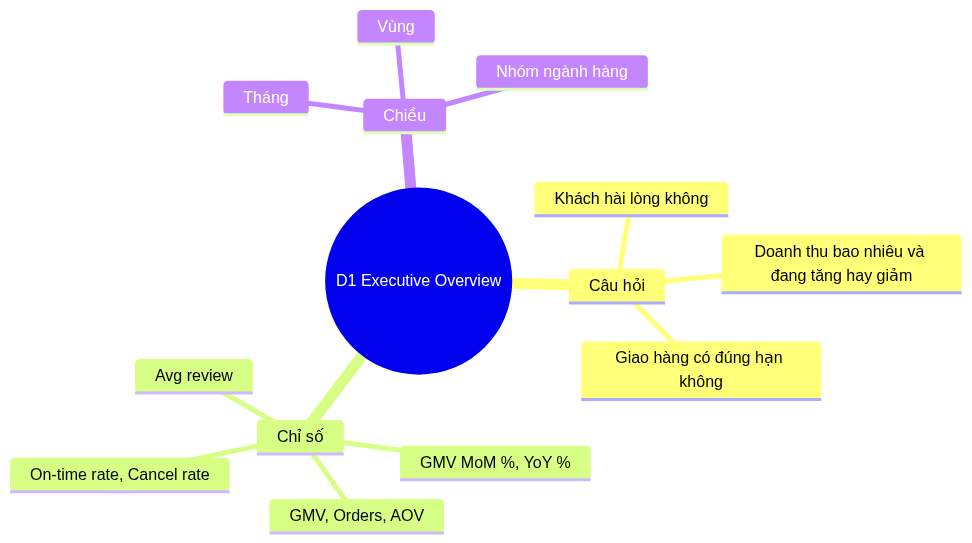
\includegraphics[width=\linewidth,height=0.3\textheight,keepaspectratio]{3-2-7_cay_phan_tich_D1.png}\end{column}\begin{column}{0.24\textwidth}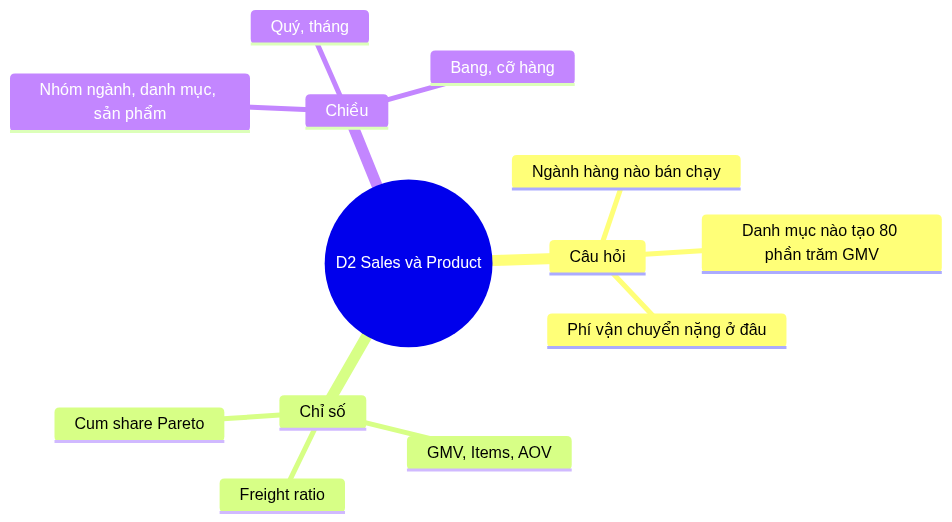
\includegraphics[width=\linewidth,height=0.3\textheight,keepaspectratio]{3-2-7_cay_phan_tich_D2.png}\end{column}\begin{column}{0.24\textwidth}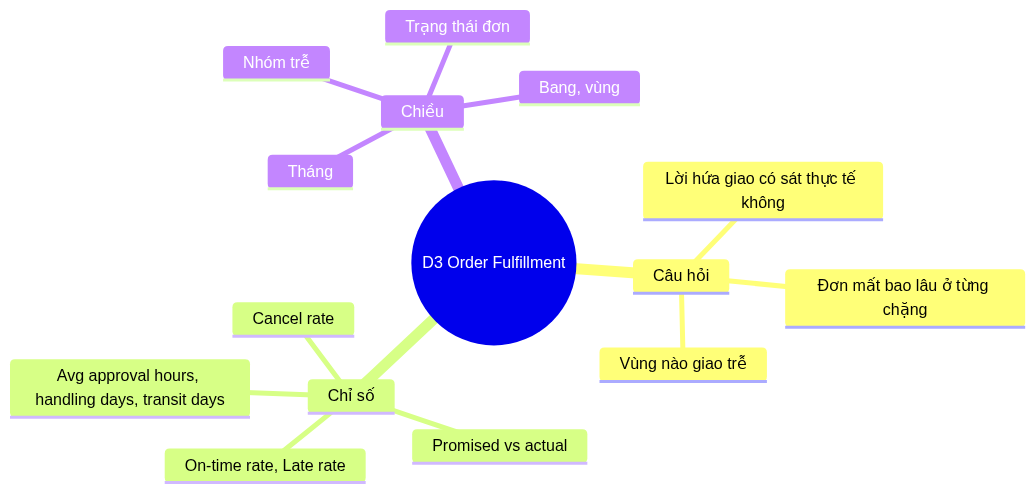
\includegraphics[width=\linewidth,height=0.3\textheight,keepaspectratio]{3-2-7_cay_phan_tich_D3.png}\end{column}\begin{column}{0.24\textwidth}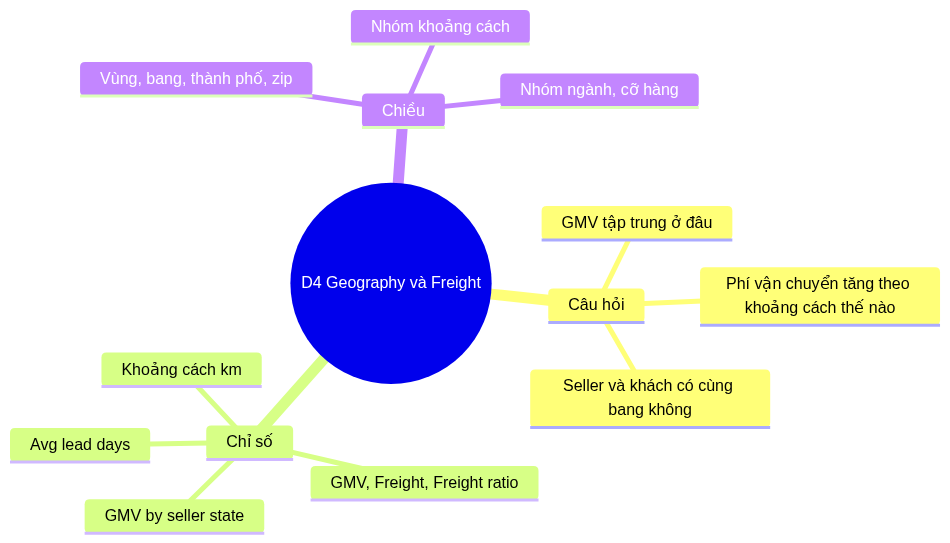
\includegraphics[width=\linewidth,height=0.3\textheight,keepaspectratio]{3-2-7_cay_phan_tich_D4.png}\end{column}\end{columns}\vspace{0.3em}\begin{columns}[c]\begin{column}{0.24\textwidth}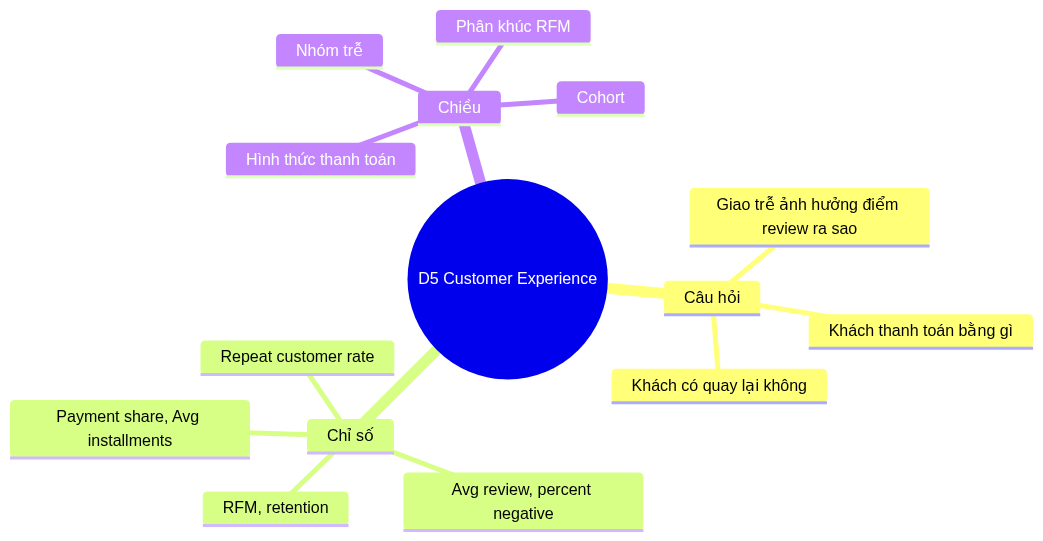
\includegraphics[width=\linewidth,height=0.3\textheight,keepaspectratio]{3-2-7_cay_phan_tich_D5.png}\end{column}\begin{column}{0.24\textwidth}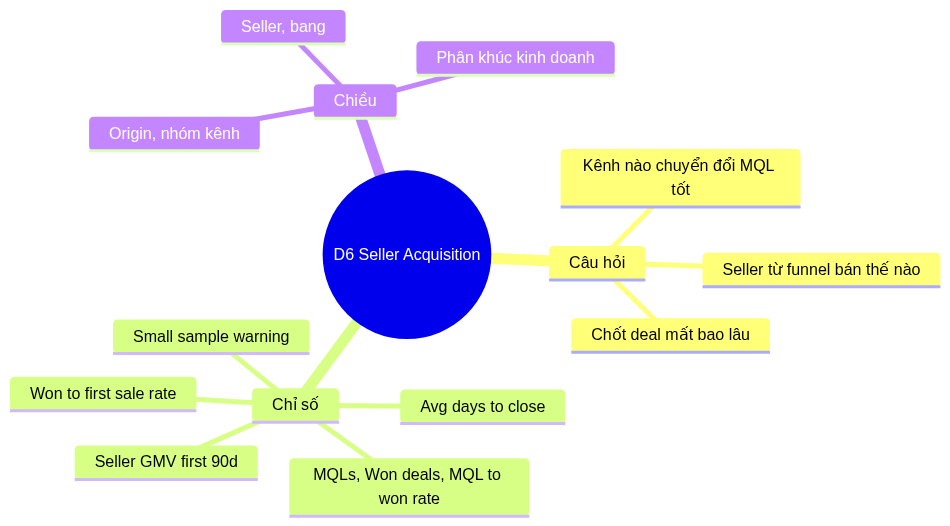
\includegraphics[width=\linewidth,height=0.3\textheight,keepaspectratio]{3-2-7_cay_phan_tich_D6.png}\end{column}\begin{column}{0.24\textwidth}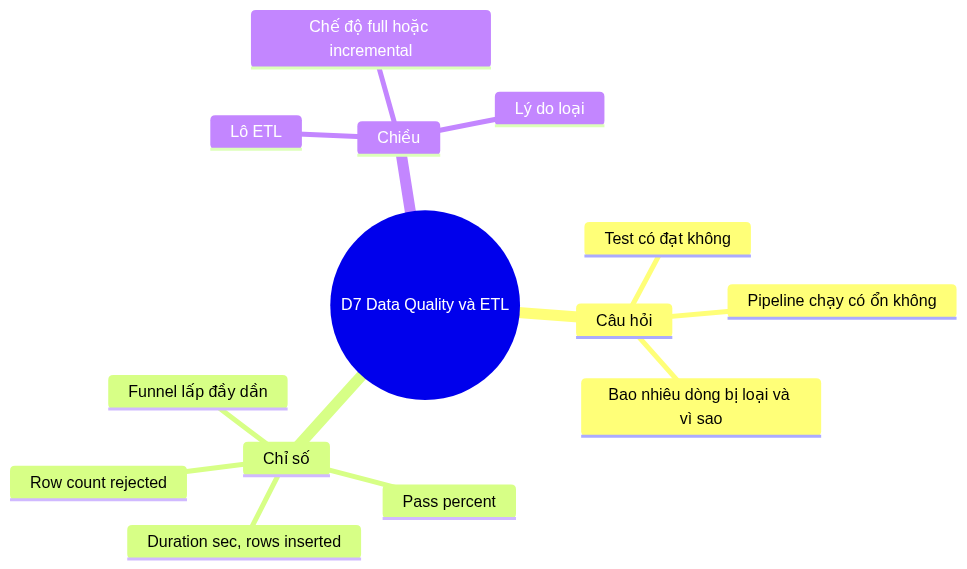
\includegraphics[width=\linewidth,height=0.3\textheight,keepaspectratio]{3-2-7_cay_phan_tich_D7.png}\end{column}\end{columns}

\note{[S31] Ví dụ D3: mục tiêu giám sát giao hàng, chỉ số on-time, promised vs actual, chiều vùng và nhóm trễ.}
\end{frame}

\begin{frame}{Phạm vi: dữ liệu 01/2017–08/2018 chiếm 99,6\% số đơn nên được dùng cho xu hướng}
\begin{columns}[T]\begin{column}{0.4\textwidth}
\begin{itemize}
  \item 2016 chỉ 329 đơn; 09–10/2018 chỉ 20 đơn
\end{itemize}
\end{column}\begin{column}{0.58\textwidth}
\begin{center}\anh[0.74\textheight]{3-3-1_orders_per_month.png}\end{center}
\end{column}\end{columns}

\note{[S32] Bộ lọc InWindow trong Power BI cố định cửa sổ này cho D1–D6.}
\end{frame}

\section[Dữ liệu và EDA]{Dữ liệu và khám phá dữ liệu}

\begin{frame}{Hai hệ thống nguồn có 11 bảng, 121 MB và 1.559.764 dòng}
\begin{itemize}
  \item oltp 9 bảng 1.550.922 dòng; crm 2 bảng 8.842 dòng
\end{itemize}
\begin{center}\adjustbox{max width=\linewidth,max height=0.5\textheight}{\scriptsize\begin{tabular}{llrrr}
\toprule
\textbf{Bảng nguồn} & \textbf{File CSV} & \textbf{Số dòng} & \textbf{Số cột} & \textbf{MB} \\
\midrule
oltp.product\_category\_name\_translation & product\_category\_name\_translation.csv & 71 & 2 & 0,00 \\
oltp.products & olist\_products\_dataset.csv & 32.951 & 9 & 2,27 \\
oltp.sellers & olist\_sellers\_dataset.csv & 3.095 & 4 & 0,17 \\
oltp.geolocation & olist\_geolocation\_dataset.csv & 1.000.163 & 6 & 58,44 \\
oltp.customers & olist\_customers\_dataset.csv & 99.441 & 5 & 8,62 \\
oltp.orders & olist\_orders\_dataset.csv & 99.441 & 8 & 16,84 \\
oltp.order\_items & olist\_order\_items\_dataset.csv & 112.650 & 7 & 14,72 \\
oltp.order\_payments & olist\_order\_payments\_dataset.csv & 103.886 & 5 & 5,51 \\
oltp.order\_reviews & olist\_order\_reviews\_dataset.csv & 99.224 & 7 & 13,78 \\
crm.mql & olist\_marketing\_qualified\_leads\_dataset.csv & 8.000 & 4 & 0,67 \\
crm.closed\_deals & olist\_closed\_deals\_dataset.csv & 842 & 14 & 0,16 \\
Tổng (11 bảng) &  & 1.559.764 &  & 121,18 \\
\bottomrule
\end{tabular}}\end{center}

\note{[S33] Vượt tiêu chí kích thước dữ liệu của môn (trên 100 MB).}
\end{frame}

\begin{frame}{Bảng toạ độ chiếm 64\% số dòng nhưng chỉ đại diện 19.015 mã bưu chính}
\begin{itemize}
  \item 1.000.163 dòng geolocation
\end{itemize}
\khungchen[0.3\textheight]{CHÈN HÌNH / BẢNG: bảng nguồn (làm nổi dòng geolocation)}

\note{[S34] Đây là bảng cần xử lý nhiều nhất ở ODS.}
\end{frame}

\begin{frame}{ERD hệ thống bán hàng: chín bảng nối quanh đơn hàng}
\begin{columns}[T]\begin{column}{0.4\textwidth}
\begin{itemize}
  \item orders $\rightarrow$ items, payments, reviews; customers, sellers, products
\end{itemize}
\end{column}\begin{column}{0.58\textwidth}
\begin{center}\anh[0.74\textheight]{3-2-4_erd_oltp.png}\end{center}
\end{column}\end{columns}

\note{[S35] \texttt{customer\_\allowbreak{}id} được sinh riêng cho từng đơn nên cần \texttt{customer\_\allowbreak{}unique\_\allowbreak{}id} để nhận ra khách thật.}
\end{frame}

\begin{frame}{Các cột được gạch chân trên ERD là cột đi sang kho, kèm ghi chú mapping}
\begin{itemize}
  \item Ví dụ: \texttt{order\_\allowbreak{}purchase\_\allowbreak{}timestamp} $\rightarrow$ \texttt{purchase\_\allowbreak{}date\_\allowbreak{}key}, \texttt{price} $\rightarrow$ \texttt{price}
\end{itemize}
\khungchen[0.3\textheight]{CHÈN HÌNH / BẢNG: ERD đã gạch chân (vẽ lại)}

\note{[S36] Bảng mapping đầy đủ 108 dòng ODS $\rightarrow$ kho nằm ở phụ lục.}
\end{frame}

\begin{frame}{Luồng dữ liệu và tần suất cập nhật: nạp ban đầu 45.430 đơn rồi 11 đợt hằng tháng}
\begin{columns}[T]\begin{column}{0.4\textwidth}
\begin{itemize}
  \item Tổng 286.144 bản ghi mới qua 11 đợt
\end{itemize}
\end{column}\begin{column}{0.58\textwidth}
\begin{center}\anh[0.74\textheight]{3-4-1_pipeline.png}\end{center}
\end{column}\end{columns}

\note{[S37] Dữ liệu Kaggle là ảnh tĩnh nên nhóm mô phỏng cập nhật.}
\end{frame}

\begin{frame}{Khám phá dữ liệu đo được 45 loại lỗi cần xử lý ở ODS}
\begin{columns}[T]\begin{column}{0.4\textwidth}
\begin{itemize}
  \item Cột thiếu, mốc thời gian sai thứ tự, tên thành phố lệch dấu, trùng lặp
\end{itemize}
\end{column}\begin{column}{0.58\textwidth}
\begin{center}\anh[0.74\textheight]{3-3-1_data_quality.png}\end{center}
\end{column}\end{columns}

\note{[S38] Không loại lỗi nào bằng cách xóa dữ liệu.}
\end{frame}

\begin{frame}{Tỷ lệ ô rỗng cho thấy cột nào cần điền unknown}
\begin{columns}[T]\begin{column}{0.4\textwidth}
\begin{itemize}
  \item Cột review và ngày giao có nhiều ô rỗng hợp lệ
\end{itemize}
\end{column}\begin{column}{0.58\textwidth}
\begin{center}\anh[0.74\textheight]{3-3-1_null_heatmap.png}\end{center}
\end{column}\end{columns}

\note{[S39] Ô rỗng của ngày giao đa phần là đơn chưa giao hoặc bị hủy.}
\end{frame}

\begin{frame}{Bảng toạ độ bẩn nhất: 93,5\% mã bưu chính có nhiều toạ độ, 26,2\% dòng trùng hoàn toàn}
\begin{columns}[T]\begin{column}{0.4\textwidth}
\begin{itemize}
  \item 7,3\% tên thành phố lệch dấu; 42 điểm ngoài lãnh thổ Brazil
\end{itemize}
\end{column}\begin{column}{0.58\textwidth}
\begin{center}\anh[0.74\textheight]{3-4-3_before_after_geolocation.png}\end{center}
\end{column}\end{columns}

\note{[S40] Giải pháp: lọc khung Brazil, lấy trung vị toạ độ và mode tên thành phố theo zip.}
\end{frame}

\begin{frame}{Phân bố giá, phí vận chuyển và lead time đều lệch phải}
\begin{columns}[T]\begin{column}{0.4\textwidth}
\begin{itemize}
  \item Nhiều giá trị lớn bất thường ở phí vận chuyển
\end{itemize}
\end{column}\begin{column}{0.58\textwidth}
\begin{center}\anh[0.74\textheight]{3-3-1_distributions_numeric.png}\end{center}
\end{column}\end{columns}

\note{[S41] Vì vậy dùng trung vị và Spearman khi cần.}
\end{frame}

\begin{frame}{Dữ liệu đơn dùng được là 01/2017–08/2018, hai đầu rất thưa}
\begin{columns}[T]\begin{column}{0.4\textwidth}
\begin{itemize}
  \item 2016 chỉ 329 đơn; 09–10/2018 chỉ 20 đơn
\end{itemize}
\end{column}\begin{column}{0.58\textwidth}
\begin{center}\anh[0.74\textheight]{3-3-1_orders_per_month.png}\end{center}
\end{column}\end{columns}

\note{[S42] Quyết định lọc thời gian đưa vào Power BI.}
\end{frame}

\begin{frame}{18/74 danh mục (24,3\%) tạo 80\% GMV, dẫn đầu health\symbol{95}beauty 9,3\%}
\begin{columns}[T]\begin{column}{0.4\textwidth}
\begin{itemize}
  \item Quy luật Pareto theo danh mục
\end{itemize}
\end{column}\begin{column}{0.58\textwidth}
\begin{center}\anh[0.74\textheight]{3-3-1_pareto_category.png}\end{center}
\end{column}\end{columns}

\note{[S43] Danh mục được gom thành 13 nhóm ngành hàng.}
\end{frame}

\begin{frame}{Seller thì phân tán hơn: 540 seller tạo 80\% GMV, 5 seller lớn nhất chỉ 7,7\%}
\begin{columns}[T]\begin{column}{0.4\textwidth}
\begin{itemize}
  \item Doanh thu không phụ thuộc vài seller
\end{itemize}
\end{column}\begin{column}{0.58\textwidth}
\begin{center}\anh[0.74\textheight]{3-3-1_pareto_seller.png}\end{center}
\end{column}\end{columns}

\note{[S44] Khác với danh mục, rủi ro tập trung vào seller thấp.}
\end{frame}

\begin{frame}{Giao trễ làm điểm review rơi từ 4,29 xuống 1,70 và 79,2\% review tiêu cực}
\begin{columns}[T]\begin{column}{0.4\textwidth}
\begin{itemize}
  \item Đơn trễ chiếm 6,5\% số review nhưng tạo 27,4\% review tiêu cực
\end{itemize}
\end{column}\begin{column}{0.58\textwidth}
\begin{center}\anh[0.74\textheight]{3-3-1_delay_vs_review.png}\end{center}
\end{column}\end{columns}

\note{[S45] Trung bình toàn sàn che mất nhóm nhỏ nhưng đau.}
\end{frame}

\begin{frame}{Trễ tập trung ở Bắc và Đông Bắc: Nordeste trễ 12,8\%, Norte lead time 22,6 ngày}
\begin{columns}[T]\begin{column}{0.4\textwidth}
\begin{itemize}
  \item Sudeste chỉ 6,1\% trễ, lead time 10,7 ngày
\end{itemize}
\end{column}\begin{column}{0.58\textwidth}
\begin{center}\anh[0.74\textheight]{3-3-1_late_rate_by_state.png}\end{center}
\end{column}\end{columns}

\note{[S46] Địa lý quyết định trải nghiệm giao hàng.}
\end{frame}

\begin{frame}{Chỉ 380/842 deal (45,1\%) có đơn: funnel và bán hàng chỉ giao nhau một phần}
\begin{columns}[T]\begin{column}{0.4\textwidth}
\begin{itemize}
  \item 380 seller tạo 674.005 BRL, 4,99\% GMV
\end{itemize}
\end{column}\begin{column}{0.58\textwidth}
\begin{center}\anh[0.74\textheight]{3-3-1_funnel_seller_overlap.png}\end{center}
\end{column}\end{columns}

\note{[S47] Quyết định D6 hiển thị cả nhóm "chốt nhưng chưa bán".}
\end{frame}

\begin{frame}{Sáu quyết định thiết kế đến từ khám phá dữ liệu}
\begin{itemize}
  \item SCD2 khách (0,26\% đổi zip); D6 hai trang; snapshot seller dày đặc; 13 nhóm ngành; zip thiếu toạ độ vẫn có dòng; mốc nạp 2017-12-31
\end{itemize}
\begin{center}\adjustbox{max width=\linewidth,max height=0.5\textheight}{\scriptsize\renewcommand{\arraystretch}{1.15}\begin{tabular}{lll}\toprule
\textbf{Quyết định} & \textbf{Nội dung} & \textbf{Số liệu đi kèm} \\\midrule
Câu a & \texttt{dim\_customer} dùng SCD2 & chỉ 0,26\% khách đổi zip \\
Câu b & D6 hai trang & 380/842 deal có đơn \\
Câu c & snapshot seller dày đặc & 36.583 so với 16.441 dòng \\
Câu d & 13 nhóm ngành hàng & 73 danh mục \\
Câu e & zip thiếu toạ độ vẫn có dòng & 168 zip, không mất đơn \\
Câu f & mốc nạp đầu 2017-12-31 & 45.430 đơn, 11 đợt sau \\
\bottomrule\end{tabular}}\end{center}

\note{[S48] Mỗi quyết định có số liệu trong \texttt{handoff/design-questions.md}.}
\end{frame}

\section[Kiến trúc và thiết kế]{Kiến trúc và thiết kế kho dữ liệu}

\begin{frame}{Kiến trúc sáu lớp từ hai hệ thống nguồn đến bảy dashboard}
\begin{columns}[T]\begin{column}{0.4\textwidth}
\begin{itemize}
  \item oltp/crm $\rightarrow$ staging $\rightarrow$ ODS $\rightarrow$ kho $\rightarrow$ data mart $\rightarrow$ Power BI; etl\_log giám sát
\end{itemize}
\end{column}\begin{column}{0.58\textwidth}
\begin{center}\anh[0.74\textheight]{3-4-1_pipeline.png}\end{center}
\end{column}\end{columns}

\note{[S49] Mỗi lớp có một việc và một cách kiểm tra riêng.}
\end{frame}

\begin{frame}{Tách lớp giúp đối soát: staging = ODS + dòng bị loại cho mọi bảng}
\begin{itemize}
  \item Chỗ nào hỏng biết ngay lớp nào
\end{itemize}
\khungchen[0.3\textheight]{CHÈN HÌNH / BẢNG: bảng đối soát (handoff P2)}

\note{[S50] Không phải lấy lại dữ liệu từ nguồn khi ODS lỗi.}
\end{frame}

\begin{frame}{Công nghệ: PostgreSQL 18, Python 3.11, SQL procedure, Power BI, Git}
\begin{itemize}
  \item Không Docker, không PostGIS; điều phối bằng một lệnh
\end{itemize}
\khungchen[0.3\textheight]{CHÈN HÌNH / BẢNG: logo công nghệ (chèn)}

\note{[S51] Chạy được trên laptop sinh viên 8 GB.}
\end{frame}

\begin{frame}{ODS là lớp làm sạch trung gian: 18 bảng, 678.183 dòng, mọi lỗi có cờ hoặc lý do}
\begin{itemize}
  \item Zip thành 5 chữ số, thành phố bỏ dấu, \texttt{NULL} thành \texttt{unknown}, khử trùng review
\end{itemize}
\begin{center}\adjustbox{max width=\linewidth,max height=0.5\textheight}{\scriptsize\begin{tabular}{p{6.2cm}rp{5.5cm}}
\toprule
\textbf{Lỗi} & \textbf{Số dòng} & \textbf{Xử lý} \\
\midrule
Bàn giao vận chuyển trước khi duyệt thanh toán & 1.359 & Gắn cờ dq\_flags, giữ đơn; khoảng thời gian âm đặt NULL \\
Bàn giao vận chuyển trước ngày mua & 166 & Gắn cờ dq\_flags, giữ đơn; khoảng thời gian âm đặt NULL \\
Giao khách trước khi bàn giao vận chuyển & 23 & Gắn cờ dq\_flags, giữ đơn; khoảng thời gian âm đặt NULL \\
Đơn đã giao nhưng không có ngày duyệt & 14 & Gắn cờ dq\_flags, giữ đơn; khoảng thời gian âm đặt NULL \\
Trạng thái delivered nhưng không có ngày giao & 8 & Gắn cờ dq\_flags, giữ đơn; khoảng thời gian âm đặt NULL \\
Có ngày giao nhưng trạng thái chưa là delivered & 6 & Gắn cờ dq\_flags, giữ đơn; khoảng thời gian âm đặt NULL \\
Đã giao nhưng không có ngày bàn giao & 2 & Gắn cờ dq\_flags, giữ đơn; khoảng thời gian âm đặt NULL \\
Giá trị thanh toán = 0 & 9 & Gắn cờ, chuẩn hoá (số kỳ 0 → 1) \\
Hình thức thanh toán not\_defined & 3 & Gắn cờ, chuẩn hoá (số kỳ 0 → 1) \\
Số kỳ trả góp = 0 (đặt thành 1) & 2 & Gắn cờ, chuẩn hoá (số kỳ 0 → 1) \\
Doanh thu tháng khai báo = 0 & 797 & Gắn cờ, giữ nguyên giá trị \\
Chốt deal trước ngày liên hệ đầu & 1 & Gắn cờ, giữ nguyên giá trị \\
coordinates outside Brazil bounding box & 42 & Loại khỏi ODS, ghi etl\_log.rejected\_rows \\
\bottomrule
\end{tabular}}\end{center}

\note{[S52] 1.411 đơn (1,4\%) có ít nhất một cờ chất lượng.}
\end{frame}

\begin{frame}{Bus matrix: sáu fact dùng chung các chiều ngày, seller, khách, địa lý}
\begin{itemize}
  \item Seller là chiều dùng chung của hai quy trình
\end{itemize}
\begin{center}\adjustbox{max width=\linewidth,max height=0.5\textheight}{\scriptsize\renewcommand{\arraystretch}{1.15}\begin{tabular}{lcccccccccc}\toprule
\textbf{Fact} & \textbf{Date} & \textbf{Customer} & \textbf{Seller} & \textbf{Product} & \textbf{Geo} & \textbf{Status} & \textbf{Payment} & \textbf{Origin} & \textbf{Profile} & \textbf{Rep} \\\midrule
fact\_order\_item & \ding{51} & \ding{51} & \ding{51} & \ding{51} & \ding{51} & \ding{51} &  &  &  &  \\
fact\_order\_fulfillment & \ding{51} & \ding{51} &  &  & \ding{51} & \ding{51} &  &  &  &  \\
fact\_payment & \ding{51} & \ding{51} &  &  &  &  & \ding{51} &  &  &  \\
fact\_review & \ding{51} & \ding{51} &  &  &  &  &  &  &  &  \\
fact\_lead\_funnel & \ding{51} &  & \ding{51} &  &  &  &  & \ding{51} & \ding{51} & \ding{51} \\
fact\_seller\_monthly & \ding{51} &  & \ding{51} &  &  &  &  &  &  &  \\
\bottomrule\end{tabular}}\end{center}

\note{[S53] Bus matrix cho thấy chiều nào được dùng lại ở đâu.}
\end{frame}

\begin{frame}{Mô hình constellation: bốn mart, sáu fact (cam), mười chiều (xanh)}
\begin{columns}[T]\begin{column}{0.4\textwidth}
\begin{itemize}
  \item Khung = data mart
\end{itemize}
\end{column}\begin{column}{0.58\textwidth}
\begin{center}\anh[0.74\textheight]{3-3-4_constellation.png}\end{center}
\end{column}\end{columns}

\note{[S54] Fact màu cam, chiều màu xanh đúng yêu cầu trình bày.}
\end{frame}

\begin{frame}{Data model logic: mỗi fact nối đúng các chiều theo bus matrix}
\begin{columns}[T]\begin{column}{0.4\textwidth}
\begin{itemize}
  \item Ví dụ \texttt{fact\_\allowbreak{}order\_\allowbreak{}item} nối 6 chiều với 2 vai địa lý
\end{itemize}
\end{column}\begin{column}{0.58\textwidth}
\begin{center}\anh[0.74\textheight]{3-3-4_erd_dw.png}\end{center}
\end{column}\end{columns}

\note{[S55] Địa lý có hai vai: khách và seller.}
\end{frame}

\begin{frame}{Data model vật lý: khoá chính theo grain, khoá ngoại có index, 112.650 dòng hàng}
\begin{columns}[T]\begin{column}{0.4\textwidth}
\begin{itemize}
  \item Mọi khoá ngoại NOT NULL, dòng Unknown -1
\end{itemize}
\end{column}\begin{column}{0.58\textwidth}
\begin{center}\anh[0.74\textheight]{3-3-4_erd_dw.png}\end{center}
\end{column}\end{columns}

\note{[S56] Tiền \texttt{numeric(12,2)}, khoá \texttt{<tên>\_\allowbreak{}key}, ngày \texttt{yyyymmdd}.}
\end{frame}

\begin{frame}{Mười bảng chiều với số dòng từ 6 đến 96.339}
\begin{itemize}
  \item dim\_date 1.828; geography 19.178; customer 96.339; seller 3.558; product 32.952; ...
\end{itemize}
\begin{center}\adjustbox{max width=\linewidth,max height=0.5\textheight}{\scriptsize\begin{tabular}{llrc}
\toprule
\textbf{Chiều} & \textbf{Grain} & \textbf{Số dòng} & \textbf{SCD} \\
\midrule
dim\_date & 1 ngày (2016-01-01 → 2020-12-31) & 1.828 & -- \\
dim\_geography & 1 mã bưu chính (zip) & 19.178 & 1 \\
dim\_customer & 1 phiên bản địa chỉ của 1 khách thật & 96.339 & 2 \\
dim\_seller & 1 seller (chiều dùng chung) & 3.558 & 1 \\
dim\_product & 1 sản phẩm & 32.952 & 1 \\
dim\_order\_status & 1 trạng thái đơn & 9 & 1 \\
dim\_payment\_type & 1 hình thức thanh toán & 6 & 1 \\
dim\_lead\_origin & 1 giá trị origin của MQL & 11 & 1 \\
dim\_lead\_profile & 1 tổ hợp thuộc tính deal (junk dimension) & 503 & -- \\
dim\_sales\_rep & 1 nhân viên và vai trò (SDR/SR) & 55 & -- \\
\bottomrule
\end{tabular}}\end{center}

\note{[S57] Mỗi chiều có đúng một dòng Unknown, được kiểm thử.}
\end{frame}

\begin{frame}{Hệ thống chiều khái niệm: phân cấp ngày, địa lý, sản phẩm, seller, khách}
\begin{itemize}
  \item Ngày $\rightarrow$ tháng $\rightarrow$ quý $\rightarrow$ năm; zip $\rightarrow$ thành phố $\rightarrow$ bang $\rightarrow$ vùng
\end{itemize}
\khungchen[0.3\textheight]{CHÈN HÌNH / BẢNG: sơ đồ phân cấp (vẽ)}

\note{[S58] Phân cấp là cơ sở của roll-up và drill-down.}
\end{frame}

\begin{frame}{SCD2 giữ lịch sử địa chỉ: 96.096 khách thành 96.339 dòng, 236 khách đổi zip}
\begin{itemize}
  \item Đơn cũ vẫn trỏ về địa chỉ lúc mua
\end{itemize}
\begin{center}\adjustbox{max width=\linewidth,max height=0.5\textheight}{\scriptsize\renewcommand{\arraystretch}{1.15}\begin{tabular}{llllllll}\toprule
\textbf{customer\_key} & \textbf{khách thật} & \textbf{zip} & \textbf{thành phố} & \textbf{effective\_from} & \textbf{effective\_to} & \textbf{is\_current} & \textbf{version} \\\midrule
15081 & 570eb70f… & 31930 & belo horizonte & 1900-01-01 & 2017-11-08 & không & 1 \\
15082 & 570eb70f… & 31130 & belo horizonte & 2017-11-09 & 9999-12-31 & có & 2 \\
\bottomrule\end{tabular}}\end{center}

\note{[S59] Ví dụ khách \texttt{570eb70f…} đổi zip ngày 09/11/2017; đơn 24/10 thuộc phiên bản 1.}
\end{frame}

\begin{frame}{dim\symbol{95}seller là chiều dùng chung: nối bán hàng với funnel qua seller\symbol{95}id}
\begin{itemize}
  \item 462 seller chỉ có trong CRM vẫn có dòng, địa chỉ Unknown
\end{itemize}
\khungchen[0.3\textheight]{CHÈN HÌNH / BẢNG: bảng ví dụ seller (\texttt{huong-dan/01-pipeline-bang-loi.md})}

\note{[S60] \texttt{first\_\allowbreak{}sale\_\allowbreak{}date} được điền sau khi nạp fact.}
\end{frame}

\begin{frame}{Chiều rác và role-playing giúp fact gọn mà vẫn đủ thông tin}
\begin{itemize}
  \item \texttt{dim\_\allowbreak{}lead\_\allowbreak{}profile} gom 7 thuộc tính thành 503 tổ hợp; \texttt{dim\_\allowbreak{}date} đóng 5 vai ở fulfillment
\end{itemize}
\khungchen[0.3\textheight]{CHÈN HÌNH / BẢNG: bảng ví dụ hai kỹ thuật}

\note{[S61] Trong Power BI, vai trò ngày dùng quan hệ không hoạt động và \texttt{USERELATIONSHIP}.}
\end{frame}

\begin{frame}{Sáu fact thuộc đủ ba loại của Kimball}
\begin{itemize}
  \item Transaction $\times$3, accumulating $\times$2, periodic $\times$1
\end{itemize}
\begin{center}\adjustbox{max width=\linewidth,max height=0.5\textheight}{\scriptsize\begin{tabular}{lllr}
\toprule
\textbf{Fact} & \textbf{Loại} & \textbf{Grain} & \textbf{Số dòng} \\
\midrule
fact\_order\_item & Transaction & 1 dòng hàng của 1 đơn & 112.650 \\
fact\_order\_fulfillment & Accumulating snapshot & 1 đơn (5 mốc thời gian) & 99.441 \\
fact\_payment & Transaction & 1 lần thanh toán & 103.886 \\
fact\_review & Transaction & 1 review của 1 đơn & 99.224 \\
fact\_lead\_funnel & Accumulating snapshot & 1 MQL & 8.000 \\
fact\_seller\_monthly & Periodic snapshot (dày đặc) & 1 seller × 1 tháng & 36.583 \\
\bottomrule
\end{tabular}}\end{center}

\note{[S62] Tổng 459.784 dòng fact (99.441 + 112.650 + 103.886 + 99.224 + 8.000 + 36.583).}
\end{frame}

\begin{frame}{fact\symbol{95}order\symbol{95}fulfillment là accumulating snapshot: một đơn một dòng, cập nhật theo mốc}
\begin{itemize}
  \item Mốc chưa xảy ra có khoá -1; thời gian từng chặng tính sẵn
\end{itemize}
\begin{center}\adjustbox{max width=\linewidth,max height=0.5\textheight}{\scriptsize\renewcommand{\arraystretch}{1.15}\begin{tabular}{ll}\toprule
\textbf{Cột của fact\_order\_fulfillment (đơn 19c36691…)} & \textbf{Giá trị} \\\midrule
approval\_hours & 36,61 \\
handling\_days & 0,71 \\
transit\_days & 12,84 \\
lead\_days & 15,07 \\
promised\_days & 21 \\
delay\_days & -6 (giao sớm 6 ngày) \\
order\_value & 43,00 \\
freight\_total & 45,30 \\
payment\_total & 88,30 \\
\bottomrule\end{tabular}}\end{center}

\note{[S63] Nếu dùng transaction fact phải ghép nhiều dòng mới tính được lead time.}
\end{frame}

\begin{frame}{fact\symbol{95}lead\symbol{95}funnel ghi lại hành trình MQL: ba mốc ngày và hai khoảng thời gian}
\begin{itemize}
  \item \texttt{days\_\allowbreak{}to\_\allowbreak{}close} TB 48,5; \texttt{days\_\allowbreak{}won\_\allowbreak{}to\_\allowbreak{}first\_\allowbreak{}sale} TB 51,8
\end{itemize}
\khungchen[0.3\textheight]{CHÈN HÌNH / BẢNG: dòng ví dụ MQL}

\note{[S64] Cũng là accumulating snapshot, 8.000 dòng.}
\end{frame}

\begin{frame}{fact\symbol{95}seller\symbol{95}monthly lưu dày đặc 36.583 dòng để thấy seller ngừng bán}
\begin{itemize}
  \item Dày đặc so với thưa: 36.583 và 16.441 dòng
\end{itemize}
\khungchen[0.3\textheight]{CHÈN HÌNH / BẢNG: bảng 4 tháng đầu của một seller}

\note{[S65] Tháng không có đơn vẫn có dòng với \texttt{orders = 0}.}
\end{frame}

\begin{frame}{Dòng Unknown -1 và khoá thay thế bảo đảm fact không bao giờ có khoá rỗng}
\begin{itemize}
  \item Mọi lỗi tra khoá được ghi \texttt{fact\_\allowbreak{}load\_\allowbreak{}issue}
\end{itemize}
\khungchen[0.3\textheight]{CHÈN HÌNH / BẢNG: bảng \texttt{dim\_\allowbreak{}seller} dòng -1}

\note{[S66] Nhờ đó ETL không làm rơi dòng khi chiều thiếu.}
\end{frame}

\section[ETL, mart, OLAP]{ETL, data mart, OLAP và hiệu năng}

\begin{frame}{Một lệnh chạy sáu bước ETL và ghi lại từng bước}
\begin{columns}[T]\begin{column}{0.4\textwidth}
\begin{itemize}
  \item extract $\rightarrow$ ODS $\rightarrow$ dim $\rightarrow$ fact $\rightarrow$ mart $\rightarrow$ tests $\rightarrow$ snapshot $\rightarrow$ export
\end{itemize}
\end{column}\begin{column}{0.58\textwidth}
\begin{center}\anh[0.74\textheight]{3-4-1_pipeline.png}\end{center}
\end{column}\end{columns}

\note{[S67] Mỗi bước ghi \texttt{job\_\allowbreak{}run}; lỗi thì dừng và đánh dấu failed.}
\end{frame}

\begin{frame}{Extract chỉ lấy dòng chưa có: đơn theo watermark, bảng nhỏ theo khoá}
\begin{columns}[T]\begin{column}{0.4\textwidth}
\begin{itemize}
  \item Chế độ full 56 giây; incremental khoảng 20 giây
\end{itemize}
\end{column}\begin{column}{0.58\textwidth}
\begin{center}\anh[0.74\textheight]{3-4-1_pipeline.png}\end{center}
\end{column}\end{columns}

\note{[S68] MQL và deal không dùng watermark ngày vì deal có thể đến trước MQL.}
\end{frame}

\begin{frame}{ODS xử lý lỗi theo ba cách: chuẩn hóa, gắn cờ hoặc loại có lý do}
\begin{itemize}
  \item 1.359 đơn bàn giao trước khi duyệt được gắn cờ, không xóa
\end{itemize}
\begin{center}\adjustbox{max width=\linewidth,max height=0.5\textheight}{\scriptsize\begin{tabular}{p{6.2cm}rp{5.5cm}}
\toprule
\textbf{Lỗi} & \textbf{Số dòng} & \textbf{Xử lý} \\
\midrule
Bàn giao vận chuyển trước khi duyệt thanh toán & 1.359 & Gắn cờ dq\_flags, giữ đơn; khoảng thời gian âm đặt NULL \\
Bàn giao vận chuyển trước ngày mua & 166 & Gắn cờ dq\_flags, giữ đơn; khoảng thời gian âm đặt NULL \\
Giao khách trước khi bàn giao vận chuyển & 23 & Gắn cờ dq\_flags, giữ đơn; khoảng thời gian âm đặt NULL \\
Đơn đã giao nhưng không có ngày duyệt & 14 & Gắn cờ dq\_flags, giữ đơn; khoảng thời gian âm đặt NULL \\
Trạng thái delivered nhưng không có ngày giao & 8 & Gắn cờ dq\_flags, giữ đơn; khoảng thời gian âm đặt NULL \\
Có ngày giao nhưng trạng thái chưa là delivered & 6 & Gắn cờ dq\_flags, giữ đơn; khoảng thời gian âm đặt NULL \\
Đã giao nhưng không có ngày bàn giao & 2 & Gắn cờ dq\_flags, giữ đơn; khoảng thời gian âm đặt NULL \\
Giá trị thanh toán = 0 & 9 & Gắn cờ, chuẩn hoá (số kỳ 0 → 1) \\
Hình thức thanh toán not\_defined & 3 & Gắn cờ, chuẩn hoá (số kỳ 0 → 1) \\
Số kỳ trả góp = 0 (đặt thành 1) & 2 & Gắn cờ, chuẩn hoá (số kỳ 0 → 1) \\
Doanh thu tháng khai báo = 0 & 797 & Gắn cờ, giữ nguyên giá trị \\
Chốt deal trước ngày liên hệ đầu & 1 & Gắn cờ, giữ nguyên giá trị \\
coordinates outside Brazil bounding box & 42 & Loại khỏi ODS, ghi etl\_log.rejected\_rows \\
\bottomrule
\end{tabular}}\end{center}

\note{[S69] Khoảng thời gian âm đặt NULL ở fact và được đếm lại.}
\end{frame}

\begin{frame}{Trước và sau ETL: bảng đơn hàng có thêm cờ lỗi và kiểu dữ liệu chuẩn}
\begin{columns}[T]\begin{column}{0.4\textwidth}
\begin{itemize}
  \item Ví dụ trước/sau
\end{itemize}
\end{column}\begin{column}{0.58\textwidth}
\begin{center}\anh[0.74\textheight]{3-4-3_before_after_orders.png}\end{center}
\end{column}\end{columns}

\note{[S70] Cùng 99.441 đơn nhưng thêm \texttt{dq\_\allowbreak{}flags}.}
\end{frame}

\begin{frame}{Trước và sau ETL: sản phẩm và seller được chuẩn hóa tên cột và thành phố}
\begin{itemize}
  \item \texttt{*\_\allowbreak{}lenght} $\rightarrow$ \texttt{*\_\allowbreak{}length}; thành phố bỏ dấu, chữ thường
\end{itemize}
\begin{columns}[c]\begin{column}{0.48\textwidth}\anh[0.46\textheight]{3-4-3_before_after_products.png}\end{column}\begin{column}{0.48\textwidth}\anh[0.46\textheight]{3-4-3_before_after_sellers.png}\end{column}\end{columns}

\note{[S71] Hai hình cùng một slide.}
\end{frame}

\begin{frame}{Trước và sau ETL: 1.000.163 dòng toạ độ gom thành 19.178 mã bưu chính}
\begin{columns}[T]\begin{column}{0.4\textwidth}
\begin{itemize}
  \item Trung vị toạ độ, mode thành phố
\end{itemize}
\end{column}\begin{column}{0.58\textwidth}
\begin{center}\anh[0.74\textheight]{3-4-3_before_after_geolocation.png}\end{center}
\end{column}\end{columns}

\note{[S72] 42 điểm ngoài Brazil được ghi vào bảng loại.}
\end{frame}

\begin{frame}{Trước và sau ETL: MQL và deal có giá trị trống thành unknown}
\begin{itemize}
  \item \texttt{origin} rỗng $\rightarrow$ \texttt{unknown}; doanh thu khai báo 0 gắn cờ
\end{itemize}
\begin{columns}[c]\begin{column}{0.48\textwidth}\anh[0.46\textheight]{3-4-3_before_after_mql.png}\end{column}\begin{column}{0.48\textwidth}\anh[0.46\textheight]{3-4-3_before_after_closed_deals.png}\end{column}\end{columns}

\note{[S73] Không đoán giá trị, chỉ đánh dấu.}
\end{frame}

\begin{frame}{Đối soát số dòng: nguồn = staging = ODS + loại, và tổng tiền khớp từng đồng}
\begin{itemize}
  \item $\Sigma$ price 13.591.643,70 BRL = file CSV
\end{itemize}
\khungchen[0.3\textheight]{CHÈN HÌNH / BẢNG: bảng đối soát (handoff P4)}

\note{[S74] Chênh lệch nếu có phải giải thích được bằng \texttt{rejected\_\allowbreak{}rows}.}
\end{frame}

\begin{frame}{SCD2 được nạp bằng window function: mỗi lần zip đổi mở một phiên bản mới}
\begin{itemize}
  \item \texttt{lag(zip)} so với đơn trước; \texttt{effective\_\allowbreak{}from} = ngày mua
\end{itemize}
\khungchen[0.3\textheight]{CHÈN HÌNH / BẢNG: đoạn SQL (Phụ lục B, \texttt{code/scd2\_\allowbreak{}dim\_\allowbreak{}customer.sql})}

\note{[S75] Khoá thay thế cũ không đổi khi chạy lại.}
\end{frame}

\begin{frame}{Nạp fact: tra khoá theo phiên bản có hiệu lực, khoảng thời gian âm thành NULL}
\begin{itemize}
  \item 1.359 đơn có \texttt{handling\_\allowbreak{}days} âm (bàn giao trước khi duyệt) được đặt NULL và đếm
\end{itemize}
\khungchen[0.3\textheight]{CHÈN HÌNH / BẢNG: bảng \texttt{fact\_\allowbreak{}load\_\allowbreak{}issue}}

\note{[S76] Tra không thấy thì dùng -1 và ghi nhận.}
\end{frame}

\begin{frame}{Nạp tăng dần mô phỏng: 11 đợt hằng tháng, tổng 286.144 bản ghi mới}
\begin{columns}[T]\begin{column}{0.4\textwidth}
\begin{itemize}
  \item \texttt{simulate\_\allowbreak{}increment} rồi \texttt{run\_\allowbreak{}pipeline --mode incremental}
\end{itemize}
\end{column}\begin{column}{0.58\textwidth}
\begin{center}\anh[0.74\textheight]{3-4-1_pipeline.png}\end{center}
\end{column}\end{columns}

\note{[S77] Đơn vào với trạng thái cuối; đó là giới hạn của mô phỏng.}
\end{frame}

\begin{frame}{Mỗi đợt chạy 20–26 giây, trong đó kiểm thử chiếm hơn một nửa}
\begin{itemize}
  \item Bảng 11 đợt: bản ghi mới, thời gian
\end{itemize}
\begin{center}\adjustbox{max width=\linewidth,max height=0.5\textheight}{\scriptsize\begin{tabular}{clrrrrrrrrr}
\toprule
\textbf{Đợt} & \textbf{Đến tháng} & \textbf{Bản ghi mới ở nguồn} & \textbf{ODS chèn} & \textbf{ODS loại} & \textbf{DW chèn / cập nhật} & \textbf{Giây} & \textbf{MQL} & \textbf{Deal} & \textbf{Seller có đơn} & \textbf{Đơn} \\
\midrule
1 & 2018-01 & 38.768 & 38.768 & 0 & 40.535 / 216 & 21,7 & 3.143 & 76 & 3 & 52.699 \\
2 & 2018-02 & 35.979 & 35.979 & 0 & 37.817 / 255 & 21,3 & 4.171 & 189 & 30 & 59.427 \\
3 & 2018-03 & 38.659 & 38.659 & 0 & 40.668 / 311 & 22,2 & 5.345 & 336 & 55 & 66.638 \\
4 & 2018-04 & 37.515 & 37.515 & 0 & 39.700 / 489 & 23,5 & 6.697 & 543 & 117 & 73.577 \\
5 & 2018-05 & 37.079 & 37.079 & 0 & 39.402 / 450 & 24,4 & 8.000 & 665 & 199 & 80.450 \\
6 & 2018-06 & 32.035 & 32.035 & 0 & 34.594 / 468 & 25,3 & 8.000 & 722 & 281 & 86.617 \\
7 & 2018-07 & 32.489 & 32.489 & 0 & 35.245 / 435 & 24,8 & 8.000 & 759 & 341 & 92.909 \\
8 & 2018-08 & 33.490 & 33.490 & 0 & 36.399 / 369 & 26,2 & 8.000 & 792 & 380 & 99.421 \\
9 & 2018-09 & 87 & 87 & 0 & 3.195 / 23 & 21,1 & 8.000 & 815 & 380 & 99.437 \\
10 & 2018-10 & 37 & 37 & 0 & 54 / 21 & 20,7 & 8.000 & 836 & 380 & 99.441 \\
11 & 2018-11 & 6 & 6 & 0 & 18 / 6 & 20,7 & 8.000 & 842 & 380 & 99.441 \\
\bottomrule
\end{tabular}}\end{center}

\note{[S78] Đợt 1–8 mang 99,95\% bản ghi mới; ba đợt cuối mang nốt 20 đơn và 50 deal.}
\end{frame}

\begin{frame}{Funnel lấp đầy dần: MQL 2.002 $\rightarrow$ 8.000, deal 3 $\rightarrow$ 842, seller có đơn 0 $\rightarrow$ 380}
\begin{itemize}
  \item Số liệu mỗi đợt từ \texttt{batch\_\allowbreak{}metrics}
\end{itemize}
\khungchen[0.3\textheight]{CHÈN HÌNH / BẢNG: biểu đồ đường từ \texttt{batch\_\allowbreak{}metrics} (dashboard D7)}

\note{[S79] Đây là điểm trình bày của nạp tăng dần.}
\end{frame}

\begin{frame}{Kết quả incremental trùng nạp full: 16/16 bảng khớp số dòng, tổng tiền và nội dung}
\begin{itemize}
  \item So sánh bằng checksum trên khoá tự nhiên
\end{itemize}
\khungchen[0.3\textheight]{CHÈN HÌNH / BẢNG: bảng so sánh (\texttt{handoff/2026-11-05-P5.md})}

\note{[S80] Khoá thay thế khác nhau nên so sánh qua khoá tự nhiên.}
\end{frame}

\begin{frame}{Dòng mồ côi được thử lại ở đợt sau, nhưng cơ chế mới được chứng minh bằng kiểm thử}
\begin{itemize}
  \item Kịch bản deal \texttt{b91cf88…} trên bản sao trong giao dịch rồi hoàn tác
\end{itemize}
\khungchen[0.3\textheight]{CHÈN HÌNH / BẢNG: sơ đồ 3 bước (loại $\rightarrow$ cha đến $\rightarrow$ nạp lại)}

\note{[S81] Trong 11 đợt thật không có dòng mồ côi nào; nhóm nói thẳng điều này.}
\end{frame}

\begin{frame}{133 phép kiểm thử đạt 100\%, cộng 5 phép đối chiếu với khám phá dữ liệu}
\begin{itemize}
  \item Số dòng, tổng tiền, grain, khoá ngoại, SCD2, mart khớp fact
\end{itemize}
\begin{center}\adjustbox{max width=\linewidth,max height=0.5\textheight}{\scriptsize\renewcommand{\arraystretch}{1.15}\begin{tabular}{ll}\toprule
\textbf{Nhóm kiểm thử} & \textbf{Số phép} \\\midrule
ODS (số dòng, loại, cleaning) & 25 \\
Dimension (Unknown, SCD2, phủ khoá) & 42 \\
Fact (đối soát, grain, khoá ngoại, logic) & 46 \\
Data mart (khớp fact) & 17 \\
Thử lại dòng mồ côi (kịch bản) & 3 \\
\textbf{Tổng} & \textbf{133 (đạt 100\%)} \\
Đối chiếu khám phá dữ liệu (chỉ báo cáo) & 5/5 khớp \\
\bottomrule\end{tabular}}\end{center}

\note{[S82] Chạy sau mỗi lần pipeline, lưu \texttt{etl\_\allowbreak{}log.dq\_\allowbreak{}check}.}
\end{frame}

\begin{frame}{Nhật ký etl\symbol{95}log cho biết mỗi lô chạy gì, mất bao lâu, loại bao nhiêu dòng}
\begin{itemize}
  \item \texttt{job\_\allowbreak{}run}, \texttt{rejected\_\allowbreak{}rows}, \texttt{dq\_\allowbreak{}check}, \texttt{batch\_\allowbreak{}metrics}
\end{itemize}
\khungchen{CHÈN ẢNH CHỤP D7}

\note{[S83] D7 là dashboard giám sát hệ thống.}
\end{frame}

\begin{frame}{Bốn data mart gồm 17 view, trong đó 4 là materialized view làm mới trong 2 giây}
\begin{itemize}
  \item Sales, fulfillment, cx, acquisition
\end{itemize}
\begin{center}\adjustbox{max width=\linewidth,max height=0.5\textheight}{\scriptsize\renewcommand{\arraystretch}{1.15}\begin{tabular}{lll}\toprule
\textbf{Mart} & \textbf{Số view} & \textbf{Dashboard} \\\midrule
mart\_sales & 6 & D1, D2, D4 \\
mart\_fulfillment & 4 & D3, D4 \\
mart\_cx & 4 (RFM, cohort materialized) & D5 \\
mart\_acquisition & 3 (scorecard, theo kênh materialized) & D6 \\
\bottomrule\end{tabular}}\end{center}

\note{[S84] Mart được làm mới tự động ở bước mart của pipeline.}
\end{frame}

\begin{frame}{Roll-up và drill-down: GMV 2017 là 6,11 triệu, 2018 là 7,34 triệu; ngày Black Friday cao gấp 5,2 lần}
\begin{itemize}
  \item Quý 4/2017: 2,41 triệu BRL; 24/11/2017: 152.654 BRL
\end{itemize}
\begin{center}\adjustbox{max width=\linewidth,max height=0.5\textheight}{\scriptsize\begin{tabular}{llrr}
\toprule
\textbf{Năm} & \textbf{Quý} & \textbf{Số đơn} & \textbf{GMV (BRL)} \\
\midrule
2017 & 2017-Q1 & 5.122 & 733.398,94 \\
2017 & 2017-Q2 & 9.222 & 1.286.918,78 \\
2017 & 2017-Q3 & 12.445 & 1.681.949,00 \\
2017 & 2017-Q4 & 17.586 & 2.406.225,55 \\
2017 & (cả năm) & 44.375 & 6.108.492,27 \\
2018 & 2018-Q1 & 20.979 & 2.764.402,78 \\
2018 & 2018-Q2 & 19.897 & 2.849.730,26 \\
2018 & 2018-Q3 & 12.655 & 1.727.049,37 \\
2018 & (cả năm) & 53.531 & 7.341.182,41 \\
Tổng & (cả năm) & 97.906 & 13.449.674,68 \\
\bottomrule
\end{tabular}}\end{center}

\note{[S85] Roll-up dùng \texttt{ROLLUP}, drill-down thêm cấp vào \texttt{GROUP BY}.}
\end{frame}

\begin{frame}{Slice, dice và pivot: vùng Sudeste chiếm 64,3\% GMV năm 2017}
\begin{itemize}
  \item Dice Sudeste $\times$ Home \& Furniture $\times$ quý 4: SP 199.179 BRL
\end{itemize}
\begin{center}\adjustbox{max width=\linewidth,max height=0.5\textheight}{\scriptsize\begin{tabular}{lrrrr}
\toprule
\textbf{Vùng} & \textbf{2016} & \textbf{2017} & \textbf{2018} & \textbf{Tổng} \\
\midrule
Sudeste & 27.701 & 3.928.343 & 4.866.293 & 8.822.336 \\
Sul & 7.456 & 883.020 & 1.047.636 & 1.938.111 \\
Nordeste & 6.013 & 727.733 & 804.568 & 1.538.314 \\
Centro-Oeste & 2.356 & 401.380 & 458.090 & 861.825 \\
Norte & 1.200 & 168.018 & 164.596 & 333.814 \\
\bottomrule
\end{tabular}}\end{center}

\note{[S86] Pivot bằng tổng có điều kiện \texttt{FILTER}.}
\end{frame}

\begin{frame}{Chọn ROLAP vì dữ liệu nhỏ, kho luôn tươi và Power BI làm lớp ngữ nghĩa}
\begin{itemize}
  \item Khác MOLAP: không phải xử lý lại khối khi nạp dữ liệu
\end{itemize}
\khungchen[0.3\textheight]{CHÈN HÌNH / BẢNG: bảng ROLAP vs MOLAP (\texttt{handoff/olap-examples.md})}

\note{[S87] Đây là lý do lựa chọn đã nêu ở phần 1.}
\end{frame}

\begin{frame}{Star schema chỉ nhanh hơn OLTP 1,0–1,6 lần; tốc độ lớn đến từ materialized view và index}
\begin{columns}[T]\begin{column}{0.4\textwidth}
\begin{itemize}
  \item Chọn lọc một seller nhanh gấp 9 lần nhờ index; materialized view dưới 1 ms so với 150–750 ms
\end{itemize}
\end{column}\begin{column}{0.58\textwidth}
\begin{center}\anh[0.74\textheight]{3-5-1_benchmark.png}\end{center}
\end{column}\end{columns}

\note{[S88] Không phóng đại: giá trị chính của mô hình chiều là truy vấn đơn giản và số liệu nhất quán.}
\end{frame}

\section[Dashboard và mở rộng]{Dashboard và mở rộng}

\begin{frame}{Bảy dashboard chia thành bốn loại: thời gian, OLAP, vận hành, thống kê}
\begin{itemize}
  \item D1 Executive $\cdot$ D2 Sales $\cdot$ D3 Fulfillment $\cdot$ D4 Geography $\cdot$ D5 Customer $\cdot$ D6 Seller $\cdot$ D7 ETL monitor
\end{itemize}
\khungchen[0.3\textheight]{CHÈN HÌNH / BẢNG: bảng 7 dashboard (\texttt{huong-dan/dashboards/})}

\note{[S89] Mỗi dashboard dùng nhiều loại biểu đồ, slicer và định dạng có điều kiện.}
\end{frame}

\begin{frame}{Mô hình Power BI có 16 bảng và 32 quan hệ, mỗi fact một quan hệ ngày hoạt động}
\begin{itemize}
  \item Quan hệ còn lại không hoạt động
\end{itemize}
\khungchen[0.3\textheight]{CHÈN HÌNH / BẢNG: ảnh chụp Model view}

\note{[S90] Tham số \texttt{DataFolder} giúp đổi máy chỉ cần sửa một giá trị.}
\end{frame}

\begin{frame}{Role-playing date và DAX tăng trưởng: GMV tháng 11/2017 tăng 52,1\% so với tháng 10}
\begin{itemize}
  \item \texttt{USERELATIONSHIP}, \texttt{DATEADD}, \texttt{SAMEPERIODLASTYEAR}
\end{itemize}
\khungchen[0.3\textheight]{CHÈN HÌNH / BẢNG: đoạn DAX (\texttt{powerbi/measures.md})}

\note{[S91] Mọi measure đối chiếu với bảng giá trị kỳ vọng từ SQL.}
\end{frame}

\begin{frame}{Chủ đề màu thống nhất: xanh là tốt, vàng cần chú ý, đỏ là xấu}
\begin{itemize}
  \item \texttt{powerbi/theme.json}; ngưỡng cảnh báo on-time 90\%/95\%
\end{itemize}
\khungchen[0.3\textheight]{CHÈN HÌNH / BẢNG: ảnh chụp theme}

\note{[S92] Cùng một quy ước màu trên mọi dashboard.}
\end{frame}

\begin{frame}{D1 Executive: GMV 13,49 triệu BRL, 98.199 đơn, đúng hạn 93,2\%, review 4,09}
\begin{itemize}
  \item Thẻ KPI, đường GMV theo tháng, cột MoM, thanh theo vùng, treemap ngành
\end{itemize}
\khungchen{CHÈN ẢNH CHỤP D1}

\note{[S93] Trang tổng quan cho lãnh đạo.}
\end{frame}

\begin{frame}{D1 cho thấy tháng 11/2017 là đỉnh (1,0 triệu BRL) và Sudeste chiếm 65\% GMV}
\begin{itemize}
  \item Black Friday 152.654 BRL trong một ngày
\end{itemize}
\khungchen{CHÈN ẢNH CHỤP D1}

\note{[S94] Từ 03/2018 GMV đi ngang nhưng cao hơn cùng kỳ (05/2018 +97\%).}
\end{frame}

\begin{frame}{D2 Sales và Product: 18 danh mục tạo 80\% GMV; Home \& Furniture dẫn đầu 22,8\%}
\begin{itemize}
  \item Treemap, ma trận drill, Pareto, scatter AOV – freight
\end{itemize}
\khungchen{CHÈN ẢNH CHỤP D2}

\note{[S95] Drill từ nhóm ngành xuống danh mục.}
\end{frame}

\begin{frame}{D2 cho thấy phí vận chuyển nặng ở hàng giá thấp và ở vùng xa}
\begin{itemize}
  \item Freight ratio 16,6\% toàn sàn
\end{itemize}
\khungchen[0.3\textheight]{CHÈN HÌNH / BẢNG: ảnh chụp D2 (scatter)}

\note{[S96] Danh mục nhẹ giá thấp bị phí vận chuyển ăn vào nhiều nhất.}
\end{frame}

\begin{frame}{D3 Order Fulfillment: lead time 12,6 ngày, phễu trạng thái và tỷ lệ trễ theo bang}
\begin{itemize}
  \item Funnel, cột chồng từng chặng, bản đồ trễ
\end{itemize}
\khungchen{CHÈN ẢNH CHỤP D3}

\note{[S97] KPI "hứa so với thực tế" nằm trên đầu trang.}
\end{frame}

\begin{frame}{D3 cho thấy Olist hứa 24,4 ngày nhưng giao 12,6 ngày: sớm hơn lời hứa 11,8 ngày}
\begin{itemize}
  \item Đúng hạn tụt 87,6\% ở Black Friday 11/2017 và 81,0\% ở 03/2018
\end{itemize}
\khungchen{CHÈN ẢNH CHỤP D3}

\note{[S98] Tải cao làm giao chậm dù trung bình vẫn "đúng hạn".}
\end{frame}

\begin{frame}{D4 Geography và Freight: Sudeste 65,4\% GMV, Norte và Nordeste chịu phí vận chuyển 22\%}
\begin{itemize}
  \item Bản đồ bong bóng, ma trận phân cấp, GMV khách và seller
\end{itemize}
\khungchen{CHÈN ẢNH CHỤP D4}

\note{[S99] Dùng \texttt{v\_\allowbreak{}geo\_\allowbreak{}state} và \texttt{v\_\allowbreak{}geo\_\allowbreak{}zip} cho bản đồ.}
\end{frame}

\begin{frame}{D4 cho thấy 36\% dòng hàng có seller và khách cùng bang}
\begin{itemize}
  \item Khoảng cách TB 598 km
\end{itemize}
\khungchen{CHÈN ẢNH CHỤP D4}

\note{[S100] Mô hình vai trò địa lý seller cho phép so sánh hai phía.}
\end{frame}

\begin{frame}{D5 Customer Experience: điểm review 4,09; 14,7\% review tiêu cực; chỉ 3,1\% khách quay lại}
\begin{itemize}
  \item Cột điểm theo nhóm trễ, donut thanh toán, RFM, cohort
\end{itemize}
\khungchen{CHÈN ẢNH CHỤP D5}

\note{[S101] Có sáu phân khúc RFM trên 94.983 khách.}
\end{frame}

\begin{frame}{D5: thẻ tín dụng chiếm 78,3\% giá trị thanh toán và trả góp trung bình 3,5 kỳ}
\begin{itemize}
  \item 66,9\% giao dịch thẻ trả góp nhiều kỳ
\end{itemize}
\khungchen{CHÈN ẢNH CHỤP D5}

\note{[S102] Boleto chiếm 17,9\%.}
\end{frame}

\begin{frame}{D6 trang 1: tỷ lệ chốt theo kênh từ 2,7\% (other) đến 16,7\% (unknown)}
\begin{itemize}
  \item Phễu MQL $\rightarrow$ deal $\rightarrow$ seller có đơn; thời gian chốt
\end{itemize}
\khungchen{CHÈN ẢNH CHỤP D6 TRANG 1}

\note{[S103] Luôn kèm cỡ mẫu: email chỉ 493 MQL.}
\end{frame}

\begin{frame}{D6 trang 2: seller từ funnel chỉ tạo 4,99\% GMV; kênh nhỏ được cảnh báo mẫu nhỏ}
\begin{itemize}
  \item Scorecard seller, GMV/seller theo kênh
\end{itemize}
\khungchen{CHÈN ẢNH CHỤP D6 TRANG 2}

\note{[S104] Email chỉ có 6 seller có đơn nên đánh dấu mẫu nhỏ.}
\end{frame}

\begin{frame}{D7 giám sát ETL: 11 đợt chạy 20–26 giây, 133 test đạt 100\%}
\begin{itemize}
  \item Thời gian theo lô, funnel lấp đầy dần, dòng bị loại theo lý do
\end{itemize}
\khungchen{CHÈN ẢNH CHỤP D7}

\note{[S105] Dòng bị loại duy nhất là 42 điểm toạ độ.}
\end{frame}

\begin{frame}{Publish to web chia sẻ cả bảy dashboard bằng một liên kết công khai}
\begin{itemize}
  \item Dữ liệu Olist công khai nên chấp nhận được
\end{itemize}
\khungchen[0.3\textheight]{CHÈN HÌNH / BẢNG: ảnh màn hình Publish to web}

\note{[S106] Nếu tài khoản bị chặn thì dùng PDF xuất từ Power BI.}
\end{frame}

\begin{frame}{Mở rộng địa lý: hàm haversine SQL thuần tính khoảng cách seller $\rightarrow$ khách cho 112.650 dòng hàng}
\begin{itemize}
  \item 555 dòng (0,49\%) thiếu toạ độ vẫn được giữ lại với giá trị trống
\end{itemize}
\khungchen[0.3\textheight]{CHÈN HÌNH / BẢNG: đoạn SQL \texttt{dw.haversine\_\allowbreak{}km} (Phụ lục B)}

\note{[S107] São Paulo – Rio tính ra 360,9 km, gần với thực tế.}
\end{frame}

\begin{frame}{Khoảng cách tăng từ dưới 100 km lên trên 1.000 km làm phí vận chuyển gấp 2,7 lần và lead time gấp 2,9 lần}
\begin{itemize}
  \item Phí 11,75 $\rightarrow$ 31,65 BRL; lead time 6,5 $\rightarrow$ 19,0 ngày; trễ 4,5\% $\rightarrow$ 10,3\%
\end{itemize}
\begin{columns}[c]\begin{column}{0.48\textwidth}\anh[0.46\textheight]{3-5-2_distance_vs_freight.png}\end{column}\begin{column}{0.48\textwidth}\anh[0.46\textheight]{3-5-2_distance_vs_leadtime.png}\end{column}\end{columns}

\note{[S108] Tương quan Spearman 0,63 với phí và 0,54 với lead time; đó là tương quan, không phải nhân quả.}
\end{frame}

\begin{frame}{Haversine thuần đủ cho khoảng cách điểm–điểm; PostGIS cần khi truy vấn bán kính hoặc đa giác}
\begin{itemize}
  \item GiST chỉ mục không gian; haversine sai số tối đa 0,5\%
\end{itemize}
\khungchen[0.3\textheight]{CHÈN HÌNH / BẢNG: bảng so sánh (\texttt{report/chapters/3-5-2-dia-ly.tex})}

\note{[S109] Nhóm không cài PostGIS nên chọn giải pháp thuần SQL.}
\end{frame}

\begin{frame}{Dựng lại toàn bộ dự án từ đầu mất 413 giây và cho kết quả giống hệt}
\begin{itemize}
  \item Xóa hai database, chạy một lệnh, 16/16 bảng khớp
\end{itemize}
\begin{center}\adjustbox{max width=\linewidth,max height=0.5\textheight}{\scriptsize\begin{tabular}{p{6cm}rp{6cm}}
\toprule
\textbf{Bước} & \textbf{Giây} & \textbf{Kết quả} \\
\midrule
drop olist\_dw + olist\_full & 0.4 & dropped \\
setup\_db (schemas, DDL, procedures, views) & 1.8 & Setup done. \\
load\_source --initial (olist\_dw, to 2017-12-31) & 15.3 & Rejected rows logged in etl\_log.rejected\_rows: 0 (batch 1) \\
load\_source --full (olist\_full) & 24.0 & Rejected rows logged in etl\_log.rejected\_rows: 0 (batch 1) \\
run\_pipeline --mode full (initial state) & 57.0 & pipeline full trên dữ liệu đến 2017-12-31: 55.9s \\
replay\_increments (11 x simulate + incremental) & 276.7 & 11 đợt hằng tháng (01/2018 → 11/2018); sau đợt cuối: 8.000 MQL, 842 deal, 380 seller có đơ \\
run\_pipeline --mode incremental (tests + export\_powerbi) & 29.5 & tests: 130/130 đạt, 0 lỗi; đối chiếu EDA 5/5 khớp \\
\bottomrule
\end{tabular}}\end{center}

\note{[S110] Khả năng tái lập là bằng chứng độ tin cậy của pipeline.}
\end{frame}

\section[Kết luận]{Kết luận}

\begin{frame}{Kết quả: một kho dữ liệu chạy được từ đầu đến cuối với 133 kiểm thử đạt và bảy dashboard}
\begin{columns}[T]\begin{column}{0.4\textwidth}
\begin{itemize}
  \item 10 chiều, 6 fact, 17 view mart; 99.441 đơn; GMV 13,49 triệu BRL
\end{itemize}
\end{column}\begin{column}{0.58\textwidth}
\begin{center}\anh[0.74\textheight]{3-3-4_constellation.png}\end{center}
\end{column}\end{columns}

\note{[S111] Tổng kết các con số chính của dự án.}
\end{frame}

\begin{frame}{Bài học: không xóa âm thầm, chọn grain trước, định nghĩa KPI một lần}
\begin{itemize}
  \item Mô hình chiều đáng dùng vì nhất quán, tốc độ đến từ materialized view và index
\end{itemize}


\note{[S112] .}
\end{frame}

\begin{frame}{Hạn chế và hướng phát triển: trạng thái trung gian của đơn, PostGIS, lịch chạy tự động}
\begin{itemize}
  \item Mô phỏng cập nhật chỉ thêm bản ghi mới; cơ chế thử lại mồ côi mới được chứng minh bằng test
\end{itemize}


\note{[S113] Nhóm nói rõ giới hạn để kết quả đáng tin.}
\end{frame}

\begin{hustdarkframe}
\centering\vspace*{0.14\paperheight}
{\Huge\bfseries\color{white} CẢM ƠN QUÝ THẦY CÔ\\VÀ CÁC BẠN ĐÃ LẮNG NGHE!\par}\vspace{1em}
{\large\color{white!85} Hỏi đáp (Q\&A)\par}\vspace{0.8em}{\normalsize\color{white!85} Nhóm \TenNhom\ -- GVHD: \GiangVien\par}
\note{[S114] Nhóm sẵn sàng trả lời; các slide dự phòng B01–B10 dùng khi cần.}
\end{hustdarkframe}


\appendix
\hustsection[panel=false]
\begin{frame}[noprogressbar,noframenumbering]{Vì sao fact\symbol{95}order\symbol{95}fulfillment là accumulating snapshot? (3)}
\begin{itemize}
  \item Đơn đi qua nhiều mốc; một dòng, cập nhật theo mốc; lead time tính sẵn (approval 10,3 giờ, handling 2,9 ngày, transit 9,3 ngày)
  \item Slide chính liên quan: S63
\end{itemize}
\begin{center}\adjustbox{max width=\linewidth,max height=0.5\textheight}{\scriptsize\renewcommand{\arraystretch}{1.15}\begin{tabular}{ll}\toprule
\textbf{Cột của fact\_order\_fulfillment (đơn 19c36691…)} & \textbf{Giá trị} \\\midrule
approval\_hours & 36,61 \\
handling\_days & 0,71 \\
transit\_days & 12,84 \\
lead\_days & 15,07 \\
promised\_days & 21 \\
delay\_days & -6 (giao sớm 6 ngày) \\
order\_value & 43,00 \\
freight\_total & 45,30 \\
payment\_total & 88,30 \\
\bottomrule\end{tabular}}\end{center}

\note{[S63] B01 - dự phòng cho câu hỏi: Vì sao \texttt{fact\_\allowbreak{}order\_\allowbreak{}fulfillment} là accumulating snapshot? (3). Xem huong-dan/04-cau-hoi-van-dap.md.}
\end{frame}

\begin{frame}[noprogressbar,noframenumbering]{Vì sao chọn ROLAP mà không MOLAP? (25)}
\begin{itemize}
  \item PostgreSQL không có khối đa chiều, dữ liệu nhỏ, kho luôn tươi, Power BI là lớp ngữ nghĩa
  \item Slide chính liên quan: S11, S87
\end{itemize}
\begin{center}\adjustbox{max width=\linewidth,max height=0.5\textheight}{\scriptsize\renewcommand{\arraystretch}{1.15}\begin{tabular}{llll}\toprule
\textbf{Tiêu chí} & \textbf{MOLAP} & \textbf{ROLAP} & \textbf{HOLAP} \\\midrule
Lưu trữ & khối đa chiều riêng & bảng quan hệ (lược đồ sao) & kết hợp hai cách \\
Tốc độ truy vấn & rất nhanh (tính sẵn) & phụ thuộc chỉ mục, materialized view & cân bằng \\
Độ tươi dữ liệu & phải xử lý lại khối & luôn tươi sau mỗi lần nạp & tùy phần \\
Công cụ & ví dụ SSAS & PostgreSQL + Power BI & -- \\
Nhóm chọn & -- & \ding{51} ROLAP & -- \\
\bottomrule\end{tabular}}\end{center}

\note{[S11] B02 - dự phòng cho câu hỏi: Vì sao chọn ROLAP mà không MOLAP? (25). Xem huong-dan/04-cau-hoi-van-dap.md.}
\end{frame}

\begin{frame}[noprogressbar,noframenumbering]{SCD2 hoạt động thế nào? (6)}
\begin{itemize}
  \item Mỗi lần zip đổi mở phiên bản mới; 96.096 khách $\rightarrow$ 96.339 dòng; fact tra theo ngày mua
  \item Slide chính liên quan: S59, S75
\end{itemize}
\begin{center}\adjustbox{max width=\linewidth,max height=0.5\textheight}{\scriptsize\renewcommand{\arraystretch}{1.15}\begin{tabular}{llllllll}\toprule
\textbf{customer\_key} & \textbf{khách thật} & \textbf{zip} & \textbf{thành phố} & \textbf{effective\_from} & \textbf{effective\_to} & \textbf{is\_current} & \textbf{version} \\\midrule
15081 & 570eb70f… & 31930 & belo horizonte & 1900-01-01 & 2017-11-08 & không & 1 \\
15082 & 570eb70f… & 31130 & belo horizonte & 2017-11-09 & 9999-12-31 & có & 2 \\
\bottomrule\end{tabular}}\end{center}

\note{[S59] B03 - dự phòng cho câu hỏi: SCD2 hoạt động thế nào? (6). Xem huong-dan/04-cau-hoi-van-dap.md.}
\end{frame}

\begin{frame}[noprogressbar,noframenumbering]{Xử lý 1 triệu dòng geolocation ra sao? (20)}
\begin{columns}[T]\begin{column}{0.4\textwidth}
\begin{itemize}
  \item Lọc khung Brazil (loại 42), trung vị toạ độ, mode thành phố, 19.015 zip; zip chỉ có toạ độ ngoài khung vẫn có dòng
  \item Slide chính liên quan: S40, S72
\end{itemize}
\end{column}\begin{column}{0.58\textwidth}
\begin{center}\anh[0.74\textheight]{3-4-3_before_after_geolocation.png}\end{center}
\end{column}\end{columns}

\note{[B04] B04 - dự phòng cho câu hỏi: Xử lý 1 triệu dòng geolocation ra sao? (20). Xem huong-dan/04-cau-hoi-van-dap.md.}
\end{frame}

\begin{frame}[noprogressbar,noframenumbering]{Vì sao đúng hạn 93,2\% mà review đơn trễ vẫn tệ? (33)}
\begin{columns}[T]\begin{column}{0.4\textwidth}
\begin{itemize}
  \item Trễ chỉ 6,8\% đơn nhưng tạo 27,4\% review tiêu cực; điểm 4,29 $\rightarrow$ 1,70; ngày dự kiến quá rộng
  \item Slide chính liên quan: S45, S98
\end{itemize}
\end{column}\begin{column}{0.58\textwidth}
\begin{center}\anh[0.74\textheight]{3-3-1_delay_vs_review.png}\end{center}
\end{column}\end{columns}

\note{[B05] B05 - dự phòng cho câu hỏi: Vì sao đúng hạn 93,2\% mà review đơn trễ vẫn tệ? (33). Xem huong-dan/04-cau-hoi-van-dap.md.}
\end{frame}

\begin{frame}[noprogressbar,noframenumbering]{Vì sao star schema chỉ nhanh hơn OLTP 1,0–1,6 lần mà vẫn đáng dùng? (30)}
\begin{columns}[T]\begin{column}{0.4\textwidth}
\begin{itemize}
  \item Dữ liệu nhỏ; giá trị là truy vấn đơn giản, KPI nhất quán; tốc độ từ materialized view và index
  \item Slide chính liên quan: S88
\end{itemize}
\end{column}\begin{column}{0.58\textwidth}
\begin{center}\anh[0.74\textheight]{3-5-1_benchmark.png}\end{center}
\end{column}\end{columns}

\note{[B06] B06 - dự phòng cho câu hỏi: Vì sao star schema chỉ nhanh hơn OLTP 1,0–1,6 lần mà vẫn đáng dùng? (30). Xem huong-dan/04-cau-hoi-van-dap.md.}
\end{frame}

\begin{frame}[noprogressbar,noframenumbering]{Làm sao biết nạp tăng dần đúng? (13)}
\begin{itemize}
  \item So với nạp full: 16/16 bảng khớp số dòng, tổng tiền, checksum; chạy lại một đợt cho 0 dòng mới
  \item Slide chính liên quan: S80
\end{itemize}


\note{[B07] B07 - dự phòng cho câu hỏi: Làm sao biết nạp tăng dần đúng? (13). Xem huong-dan/04-cau-hoi-van-dap.md.}
\end{frame}

\begin{frame}[noprogressbar,noframenumbering]{GMV khác tổng giá hàng thế nào? (23)}
\begin{itemize}
  \item GMV loại đơn Failed: 13.494.400,74 so với 13.591.643,70
  \item Slide chính liên quan: S26, S30
\end{itemize}


\note{[B08] B08 - dự phòng cho câu hỏi: GMV khác tổng giá hàng thế nào? (23). Xem huong-dan/04-cau-hoi-van-dap.md.}
\end{frame}

\begin{frame}[noprogressbar,noframenumbering]{Dòng mồ côi được xử lý ra sao? (15)}
\begin{itemize}
  \item Loại kèm lý do, thử lại ở đợt sau; mới chứng minh bằng test
  \item Slide chính liên quan: S81
\end{itemize}


\note{[B09] B09 - dự phòng cho câu hỏi: Dòng mồ côi được xử lý ra sao? (15). Xem huong-dan/04-cau-hoi-van-dap.md.}
\end{frame}

\begin{frame}[noprogressbar,noframenumbering]{Ngày hứa giao so với thực tế cho thấy điều gì? (34)}
\begin{itemize}
  \item Hứa 24,4, thực tế 12,6: sớm 11,8 ngày; 91,9\% đơn giao sớm
  \item Slide chính liên quan: S27, S98
\end{itemize}


\note{[B10] B10 - dự phòng cho câu hỏi: Ngày hứa giao so với thực tế cho thấy điều gì? (34). Xem huong-dan/04-cau-hoi-van-dap.md.}
\end{frame}

\end{document}
